\documentclass{thesisclass}
% Based on thesisclass.cls of Timo Rohrberg, 2009
% ----------------------------------------------------------------
% Thesis - Main document
% ----------------------------------------------------------------


%% -------------------------------
%% |  Information for PDF file   |
%% -------------------------------
\hypersetup{
 pdfauthor= {Philipp Rovedo}
 pdftitle= {Muon induced secondary electrons at the KATRIN experiment}
 pdfsubject= {}
 pdfkeywords= {}
}


%% ---------------------------------
%% | Information about the thesis  |
%% ---------------------------------

\newcommand{\myname}{Philipp Rovedo}
\newcommand{\mytitle}{Muon induced secondary electrons at the KATRIN experiment\\Detector installation and setup \& data analysis}
\newcommand{\myinstitute}{IKP - Institut fuer Kernphysik - KIT Karlsruhe} 

\newcommand{\reviewerone}{Prof. Dr. Guido Drexlin}
\newcommand{\reviewertwo}{Prof. Dr. Ulrich Husemann}
\newcommand{\advisor}{Nancy Wandkowsky}
\newcommand{\advisortwo}{?}

\newcommand{\timestart}{ September 27th 2012}
\newcommand{\timeend}{ September 27th 2013}
\newcommand{\submissiontime}{DD. MM. 20XX}


%% ---------------------------------
%% | ToDo Marker - only for draft! |
%% ---------------------------------
% Remove this section for final version!
\setlength{\marginparwidth}{20mm}

\newcommand{\margtodo}
{\marginpar{\textbf{\textcolor{red}{ToDo}}}{}}

\newcommand{\todo}[1]
{{\textbf{\textcolor{red}{(\margtodo{}#1)}}}{}}


%% --------------------------------
%% | Old Marker - only for draft! |
%% --------------------------------
% Remove this section for final version!
\newenvironment{deprecated}
{\begin{color}{gray}}
{\end{color}}


%% --------------------------------
%% | Settings for word separation |
%% --------------------------------
% Help for separation:
% In german package the following hints are additionally available:
% "- = Additional separation
% "| = Suppress ligation and possible separation (e.g. Schaf"|fell)
% "~ = Hyphenation without separation (e.g. bergauf und "~ab)
% "= = Hyphenation with separation before and after
% "" = Separation without a hyphenation (e.g. und/""oder)

% Describe separation hints here:
\hyphenation{
% KaLi::KL-Energy-Events
% Pro-to-koll-in-stan-zen
% Ma-na-ge-ment  Netz-werk-ele-men-ten
% Netz-werk Netz-werk-re-ser-vie-rung
% Netz-werk-adap-ter Fein-ju-stier-ung
% Da-ten-strom-spe-zi-fi-ka-tion Pa-ket-rumpf
% Kon-troll-in-stanz
}

\usepackage[separate-uncertainty=true]{siunitx}
\usepackage{multirow, graphicx}
\usepackage{caption}
\usepackage{tabularx}
\usepackage{longtable}
\usepackage{rotating} 
%\usepackage{subcaption}
\usepackage{amsmath}
\usepackage[version = 3]{mhchem}
%\usepackage{beramono}
\usepackage{microtype,textcomp}
\usepackage{url}
\usepackage{supertabular}
\usepackage{nth}
\DeclareSIUnit\gauss{G}
\DeclareSIUnit\year{a}
\DeclareSIUnit\CL{C.L.}
\DeclareSIUnit\cps{cps}

\newcolumntype{L}[1]{>{\raggedright\let\newline\\\arraybackslash\hspace{0pt}}m{#1}}
\newcolumntype{C}[1]{>{\centering\let\newline\\\arraybackslash\hspace{0pt}}m{#1}}
\newcolumntype{R}[1]{>{\raggedleft\let\newline\\\arraybackslash\hspace{0pt}}m{#1}}
%\sisetup{math-micro=\text{µ},text-micro=µ}

%% ------------------------
%% |    Including files   |
%% ------------------------
% Only files listed here will be included!
% Userful command for partially translating the document (for bug-fixing e.g.)
\includeonly{
titlepage,
declaration,
content,
introduction,
theKATRINexperiment/theKATRINexperiment,
muonDetectionSystem/muonDetectionSystem,
analysisSoftware/analysisSoftware,
analysis/analysis,
simulationSoftware/simulationSoftware,
%evaluation,
%
conclusion,
appendix
}


%%%%%%%%%%%%%%%%%%%%%%%%%%%%%%%%%
%% Here, main documents begins %%
%%%%%%%%%%%%%%%%%%%%%%%%%%%%%%%%%
\begin{document}

% Remove the following line for German text
\selectlanguage{english}

\frontmatter
\pagenumbering{roman}
\include{titlepage}
\blankpage
\vspace*{36\baselineskip}
\hbox to \textwidth{\hrulefill}
\par
Ich versichere wahrheitsgem\"a\ss, die Arbeit selbstst\"andig angefertigt, alle benutzten Hilfsmittel vollst\"andig und genau angegeben und alles kenntlich gemacht zu haben, was aus Arbeiten anderer unver\"andert oder mit Ab\"anderungen entnommen wurde.

\textbf{PLACE, DATE}
\vspace{1.5cm}

\dotfill\hspace*{8.0cm}\\
\hspace*{2cm}(\textbf{YOUR NAME}) %center name with hspace

\thispagestyle{empty}
\blankpage


%% -------------------
%% |   Directories   |
%% -------------------
\tableofcontents
\blankpage


%% -----------------
%% |   Main part   |
%% -----------------

\listoffigures
\listoftables
\mainmatter
\pagenumbering{arabic}
%% introduction.tex
%%

%% ==============================
\chapter{Introduction}
\label{ch:Introduction}
%% ==============================
    \section{Neutrinos in the standard model}
    \label{ch:Introduction:sec:Neutrinos in the standard model}
    During the second part of the 20th century, a model stating 16 particles has been developed to describe a huge portion of known phenomena, the standard model. It contains six quarks, six leptons (both made up of three particle generations) and four types of Gauge Bosons. The latter are carriers of the standard models interactions of the former particles, meaning all interactions of matter are based on the exchange of one or more of the Gauge Bosons. 
    For our universe, gravity, the graviton generated force, plays a major role for formation and stability af almost all larger structures. In particle physics however, it can mostly be neglected. Here, only the strong and weak as well as the electromagnetic interaction make for noticable contributions to phenomena observed. That is why, in the standard model, gravity as well as its carrier, the graviton, are neglected.
    Most of what we can observe with our bare eyes or in basic experiments is attributable to the electromagnetic force or gravity, however, strong and weak interaction do play a major role when it comes to high energy physics. Here, the limited reach of the two is overcome by small distances between interacting particles. In case of the neutrino, detection and by that the study of its characteristics is even more difficult as it interacts only gravitationally and weakly. Now, as mentioned before, gravity is indeed long range, but very weak in force. And although weak intraction is a lot stronger compared to gravity, it is still weak compared to both electromagnetic and strong interactions. That is why the neutrino is considered elusive, detection efficiencies are low and only large scale detectors are able to detect statistically relevant amounts of neutrinos.
    One method used quite frequently is the Cherenkov radiation emitted while travelling through matter at speeds above the speed of light. This light, comparable to the supersonic cones planes cause in air, can be detected by standard photomiltiplier tubes. The problem is that, as mentioned above, the volumes to be able to make dependable statements on directions and energies need to be large. This is why most experiments make use of ``natural'' detectors such as water \todo{cite MARE+ICE Cube} or even ice.
    Other approaches are to catch neutrinos in reactions where those are required such as inverse beta decays:
    \begin{equation}
		\ce{\bar\nu_e + p -> e^+ + n}
    \end{equation}
   
    
    In the standard model, neutrinos are considered massless. 
    Many experiments though have shown that the weightless neutrino is a wrong assumption. Most of these were experiments prooving neutrino oscillatinos with both reactor neutrinos and solar neutrinos such as Kamiokande\cite{PhysRevLett.110.181802} or SNO \cite{SNOOscillations} \todo{add experiments}.
    Important for those experiments is the known source location making baseline analysis possible.
    
    Up till now, only the differences of the squared masses are known. This leads to different relations depending on how masses are distributed between the flavours, \ref{fig:massSchemes}, and how large they are absolutely \ref{fig:massHierarchy}. This problem is solved by the knowledge of one of the masses. KATRIN is on the verge of finding the $\nu_e$'s mass.\cite{becker2008a}
    
    \begin{figure}
    \centering
    \includegraphics[width=0.5\textwidth]{graphics/standardModel/massHierarchy.jpg}
    	 \caption[Neutrino mass hierarchy]{The possible mass hierarchies for neutrinos.}
    	\label{fig:massSchemes}
    \end{figure}
    \begin{figure}
	\caption[Neutrino mass areas]{Possible mass areas}
    	\label{fig:massHierarchy}
    \end{figure}

    
    \subsection{Neutrino Oscillations}
    \label{ch:Introduction:sec:Massive neutrino:subsec:neutrino Oscillations}
      If the neutrinos were without mass, its mass eigenstates would equal its flavour eigenstates:
      
    \begin{equation}
	\begin{array}{ccc}
      	|\nu_e>		& = & |\nu_1>\\
      	|\nu_\mu>	& = & |\nu_2>\\
      	|\nu_\tau>	& = & |\nu_3>\\
    	 \end{array}
    \end{equation}
    First doubts concerning this asumptions occured as inconsistencies between the measured and the calculated solar $\nu$-flux occured. As the count on $\nu_e$ was too low, the theory of neutrino oscillations emerged, stating that a mixture of flavours was possible as the flavours were made up of all three of the mass eigenstates. The mixture is described by the so called Pontecorvo-Maki-Nakagawa-Sakata matrix:
        \begin{equation}
        \left(
        \begin{array}{c}
	  |\nu_e>\\
	  |\nu_\mu>\\
	  |\nu_\tau>\\
        \end{array}
        \right)
	 = \left(
	\begin{array}{ccc}
      	\theta_{e,1} & \theta_{e,2} & \theta_{e,3}\\
      	\theta_{\mu,1} & \theta_{\mu,2} & \theta_{\mu,3}\\
      	\theta_{\tau,1} & \theta_{\tau,2} & \theta_{\tau,3}\\
      	\end{array}
	\right)
	\left(
	\begin{array}{c}
      	|\nu_1>\\
      	|\nu_2>\\
      	|\nu_3>\\
    	 \end{array}
    	 \right)
    \end{equation}
    
    \subsection{Direct measurement of neutrino mass}
    \label{ch:Introduction:sec:Massive neutrino:subsec:direct Neutrino Mass measurement}
    Direct measurements of the neutrino mass require a reaction known to include neutrinos in its equation. There are both spectrometric and calorimetric approaches. While the scale of spectrometers is getting bigger and bigger, calorimetric approaches seem to be a reasonable alternative, although the slow detector response - the detector material itself is decaying - requires for large arrays of detectors leading to extensive space requirements as well at some point. The luminosity of spectrometer experiments though is unachieved by any other. That is why the KATRIN collaboration is working on a setup to measure electrons from Tritium decay to determine the neutrino mass. 
     
    \subsection{Indirect measurement of neutrino mass}
    \label{ch:Introduction:sec:Massive neutrino:subsec:indirect Neutrino Mass measurement}
    Another approach is using indirect ways of finding the neutrino mass. One possibility here is to search for neutrinoless double beta decay, $0\nu\beta\beta$, which can exist only if the neutrino is its own anti-particle, a so called majorana neutrino. Then, if two nuclei beta decay, the neutrino from one vertex can be absorbed in the second as an anti-neutrino - or vice versa. The decay would then not emit any neutrino and the rate would be dependant on the effective Majorana neutrino mass square'' \cite{currentNeutrinoSearches}:
    \begin{equation}
    	\Gamma_{0\nu\beta\beta} \propto \left| \sum{U_{ei}^2m\left(\nu_i\right)}\right|^2
    \end{equation}

    
    \section{Cosmic muons and their interaction with matter}
    \label{ch:introduction:sec:Cosmic Air Showers}
    When high energy particles hit the upper parts of the atmosphere, a cascade of particles generated from the interaction with atmospheric molecules and atoms follows. Most primary particles are nucleons, most of which again are free protons, i.e. Hydrogen ions. Helium nucleons' fluxes are already about a order of magnitude below that, higher mass number nuclei show even lower rates\cite{highEnergyCosmicRays}. 
    \begin{figure}
	\begin{minipage}[d]{0.49 \textwidth}
		  \includegraphics[width=\textwidth]{graphics/cosmicRays/cosmicRays.jpg}
	\end{minipage}
	\begin{minipage}[d]{0.49 \textwidth}
		  \includegraphics[width=\textwidth]{graphics/cosmicRays/energySpectrum.jpg}
	\end{minipage}
	\caption[Cosmic ray composition]{On the left, an artistic impression of various cosmic rays hitting the atmosphere \cite{airShower}. On the right, the measured composition for cosmic nuclei is shown: on top, the lightest particle, the proton. further down, all with orders of magnitude smaller rates, heavier ions.}
    \end{figure}
    \todo{insert right side graphic from TODOR}
    By different interactions, secondary partcles are created. Any particle satisfying the inequation \begin{equation}
      E_{sec,kin} + m_{sec} c^2 < E_{prim,kin} + m_{prim}
    \end{equation}
    can be created. Mostly pions at first, those cascade further. Often through intermediate photons, muons emerge. These travel towards the earths surface mostly close to the speed of light due to their small masses though high energies. Even at these high speeds, the muons' average decay time of around \SI{2.2}{\micro\second} \cite{muonLifetime} is too small for many muons to reach the earth's surface from our reference frame's point of view. In the most common production height of \SI{2}{\kilo\meter} \cite{muonProductionHeight}, the non relativistic time of flight for a \SI{90}{\percent} speed of light particle would be
    \begin{equation}
	t_{class} = \SI{2}{\kilo\meter} / 0.9\cdot c = 
    \end{equation}
    meaning only time dilation from special relativity makes the muon flux as large as ist is:
    \begin{equation}
    	t_{rel} = t_{class} / \sqrt{1-0.9^2}
    \end{equation}
    which, from our reference frame, prolongs the lifetime by a factor of around 5, being already enough to reach the surface from heights of \SI{3}{\kilo\meter}. Most muons have even higher energies, making it possible for them to reach surface from greater heigts and under non perpendicular angles towards it.
    For KATRIN, this poses a problem. A smaller flux would be advantageous, as muons may, through different kinds of interaction, cause emission of electrons from the spectrometer vessels surface. Shielding against muons is difficult as it requires thick layers of dense matter due to the muons high energies and the low deposition in matter in relations to those. 
    



% theKATRINexperiment.tex
%

    \chapter{KATRIN experiment}
    \label{ch:The KATRIN experiment}
    The KATRIN experiment is on its way to measure the neutrino mass or set new upper limits at precisions never achieved before. It will reach a sensitivity of \SI{200}{\milli\electronvolt}/\SI{}{\square c} at \SI{90}{\percent} C.L. excelling the previously best experiments of Mainz and Troisk by a factor of \SI{10}{}. Major challenges of the project are the requirement of ultra high vacuum, the exact knowledge of all magnetic and electric fields as well as external influences on those, the required high luminosity of the tritium source and the classification and reduction of background sources.
    
      \section{Measurement principle}
      \label{ch:The KATRIN experiment:sec:Measurement Principle}
      A generally easy principle is used to find information on the neutrino mass. The energy of electrons from tritium decay is measured with high precision and compared to the standard model's presumption for a massless neutrino \cite{}
      \begin{equation}
      	\ce{^3_1T -> ^3_1H^+ + e^- + \bar{\nu}_e}.
      \end{equation}
      As the decay's energy is distributed between the constant neutrino's rest mass and the neutrino's and the electron's kinetic energies respectively, the decay electrons will show a continuous spectrum. The difference between the electron energy calculated by standard model presumptions and the extrapolated maximum electron energy from the spectrum is extracted. As all three mass eigenstates contribute to the electron neutrino's mass in any scenario (see \ref{ch:Introduction:sec:neutrino Oscillations}, the difference will be a superposition of these. The knees occuring at each single eigenstates mass can not be resolved with the KATRIN spectrometer as the energy resolution is larger than the root of the squared mass differences.
      shown in figure \ref{fig:katrinExperiment:tritiumSpectrum}. As all three flavors contribute to the electron neutrino's mass, what will be measured is the incoherent sum of all three as described in chapter \ref{ch:Introduction:sec:Neutrinos in the standard model}.
      
      \begin{figure}
	\centering
      	\includegraphics[width = 0.9 \textwidth]{graphics/katrinExperiment/electronSpectrum.jpg}
      	\caption[Schematic tritium energy spectrum]{Schematic energy spectrum for electrons from tritium beta decay. On the left, the entire spectrum with the peak at the energy most emitted - around \SI{5}{\electronvolt} - can be seen. On the right, a zoom-in on the endpoint showing both the calculations for a massless and a \SI{1}{\electronvolt} neutrino. As described in the graph, rates in this region are extremely low and extrapolation through advanced software tools needs to be applied.}
      	\label{fig:katrinExperiment:tritiumSpectrum}
      \end{figure}
      A different light is shed on the simplicity of the task when considering the needed accuracy of $\Delta E < \SI{0.93}{\electronvolt}$ needed for the electrostatic filter to achieve the desired sensitivity \cite{KATRINWolf}. And this is just one in a meshwork of requirements necessary. All components need to work as a whole in the end, not a single one may contribute to the background much more than expected.
       \subsection{MAC-E Filter}
      \label{ch:The KATRIN experiment:sec:MAC-E}
		To measure the energy of electrically charged decay electrons at high precision, an electrostatic filter comes to mind. As the electrons are emitted isotropically, they will have momentum components both parallel and perpendicular to the source-detector axis (defined as the z-axis). To make statements on the overall energy, the momentum direction needs to be well defined. In case of an electrostatic filter, it needs to be parallel to the electric field to be analyzed.
		At the same time, a high luminosity is a major requirement for good statistics for the KATRIN experiment.
		To satisfy all these requirements, several techniques are combined in the MAC-E filter - magnetic adiabatic collimation with electrostatic filter.\\
		{\bf Magnetic} fieldlines connect the source and the detector. Electrons from tritium decays are guided from source side to detector in cyclotron motion around one of these field lines. This strongly raises luminosity as electrons with large angles towards the z axis will not necessarily hit the wall of the source but will be able to reach the detector.\\
		{\bf Adiabatic} motion in the magnetic field is defined by the allowance of momentum direction changes at constant momentum value. That is given if the magetic field change is small within each cyclotron orbit. If so, the magnetic momentum $\mu$ correlated to $E_\bot$, the energy perpendicular to the magnetic field $B$, as follows remains constant
		\begin{equation}
			\mu = \frac{E_{\bot}}{B} = const \propto \frac{p_\bot}{B}.
			\label{eq:magMomentum}
		\end{equation}
		{\bf Collimation} in a MAC-E filter is based on the above adiabacity. Magnetic field strengths drop over several orders of magnitude from $B_{max}$ at the solenoid magnets to $B_{min}$ in the analysis plane (see figure \ref{fig:katrinExperiment:macEFilter}). Considering equation \ref{eq:magMomentum}, this means that the energy perpendicular to the magnetic field must drop over the same order of magnitude for $\mu$ to remain constant.\\
		{\bf Electrostatic} filtering occurs exactly at that point of minimal energies $E_\bot$ in the analysis plane. Here, the momentum vector is mostly defined by its component parallel to the magnetic field $E_{||}$. Setting the electrostatic filter to a fixed voltage $U$ now reflects electrons with $E_{||} < Ue$.\\
		Most electrons are emitted at the source are non-parallel to the magnetic field lines and thus an energy $E_\bot \neq 0$. That means that it is very likely that electrons in the analysis plane have remaining energy $E_\bot$. This limits the filter resolution, the relative sharpness is given by
		\begin{equation}
		\Delta E = E_{\bot_{max}} = E_{\bot_0}\frac{B_{low}}{B_{0}}
% 			\frac{\Delta E}{E} = \frac{B_{min}}{B_{max}}.
		\end{equation}
		Only in the edge case of $B\rightarrow 0$ in the analysing plane, the momentum would need to be exactly parallel to the field and the resolution would not be limited. The resolution also depends on the choice of accepted starting angles. 
		\begin{equation}
			\mu_{\mathrm{0}} = \mu_{\mathrm{low}} ~ \longrightarrow ~ \frac{E_{\bot_0}}{B_0} = \frac{E_{\bot_{low}}}{B_{low}} 
		\end{equation}
      
      
      To further filter out electrons with high starting angle, the source is set to lower fields than the maximum $B_{max}$.
      As with larger angles come longer paths, this reduces the probability of electrons taking part in scattering processes inside the source section being detected.
      \begin{equation}
      	\theta_{s~max}= \arcsin{\sqrt{\frac{B_s}{B_{max}}}}
      \end{equation}
      With the chosen settings This results in an angular acceptance of 2$\pi$.
      
      The main spectrometer reaches a resolution of \SI{0.93}{\electronvolt}.
            \begin{figure}
	\centering
      	\includegraphics[width = 0.6 \textwidth]{graphics/katrinExperiment/macEFilter.jpg}
      	\caption[MAC E Filter]{Principle of a MAC E filter. The angular momentum of an electron not starting parallel to the magnetic field lines is converted mostly to linear kinetic energy up to the point of lowest fields. Here, the energy is analyzed before the particle is guided towards the detector \cite{macEFilter}.}
      	\label{fig:katrinExperiment:macEFilter}
      \end{figure}
      

      \section{Experimental Setup}
      \label{ch:The KATRIN experiment:sec:Experimental setup}
      The KATRIN experiment is made up of different sections all fulfilling their own important purpose in the whole setup. All begins at the windowless gaseous tritium source ``WGTS''. Here, tritium decays isotropically emitting electrons. These are guided magnetically through the differential and cryogenic pumping sections ``DPS'' and ``CPS'' removing hydrogen ions and other residual gases in the process. At the same time, looking at the WGTS from the other direction, the rear section scans the activity of the source. For the electrons on their way to the detector, the path continues through the two spectrometers posing as a energetic high pass filter to the focal plane detector ``FPD'' registering them.\\
      During the whole procedure, the electrons from the decay may not undergo energy changes as the knowledge of their kinetic energy after decaying is essential to the experiment. That is why the guiding needs to be adiabatic. This is guaranteed by spatially slowly changing and timewise very constant magnetic fields.\\
      See figure \ref{fig:beamLine} for a schematic overview of the whole experimantal setup. It follows a more detailed description of the individual components.
      
      \begin{figure}
			
      		\includegraphics[width = \textwidth]{graphics/katrinExperiment/beamLineHD.jpg}

      	\caption[KATRIN beam line]{The beam line of the KATRIN experiment with the different stages: Rear section (yellow) and WGTS (blue) on the very left, followed by the transport section (red) consisting of DPS and CPS. Energy analysis in pre- (green) and main spectrometer (grey-red) of the spectrometer section and electron detection at the detector section (grey-blue).}
      	\label{fig:beamLine}
      \end{figure}

      
      \subsection{WGTS and Rear Section}
      \label{ch:The KATRIN experiment:sec:Experimental setup:subsec:sourceSide}
      To generate tritium decay electrons, a gaseous tritium source is utilized (see figure \ref{fig:sourceSide}). Advantages of the principle are the absence of solid state effects and a high luminosity \cite{letterOfIntent}. In a solid, like tritium films, most electrons from decays inside the structure would interact with the solid itself. That could lead to energy shifts threatening the energy resolution. Another advantage of using a gaseous source is that not only the surface facing the detector emits electrons at the required spectrum, but the electrons from the whole volume covered by the magnetic flux tube hitting the detector can be analyzed. Furthermore, the emission of this kind of source is very homogeneous. Of course, new challenges arise from the decision to use gas instead of solids.
      \begin{itemize}
		\item The source's temperature needs to be very robust (max. \SI{\pm0.03}{\kelvin} at \SI{30}{\kelvin}) to guarantee a rate stability of \SI{\pm0.1}{\percent} for the decay electrons \cite{temperatureWGTS}.
      	\item The spectrometers further downstream require for ultra high vacuum, for the main spectrometer in the order of \SI{e-11}{\milli\bar}. With the tritium pressure is in the order of \SI{10e-3}{\milli\bar} and the source's need to be windowless - no electron transparent window is known to stand such pressure differences - the pressure must be reduced to desired values without any physical barrier.
      	\item The tritium isotope contributions of the gas need to be known precisely, for that purpose a laser-raman-system has been developed \cite{calibrationRaman}.
      	\item All devices used in contact with tritium have to undergo excessive testing in tritium environment to fault failure safety under the harsh conditions.
      \end{itemize}
      
     \begin{figure}
     \centering
		\begin{minipage}{0.6\textwidth}
				\includegraphics[width = 1.0\textwidth]{graphics/katrinExperiment/rearSectionFull1.png}
		\end{minipage}
		\begin{minipage}{\textwidth}
			\includegraphics[width = 1.0\textwidth]{graphics/katrinExperiment/WGTS.jpg}
		\end{minipage}
		\caption[Rear section and WGTS]{On top, the rear section. In the model, there are two large attachments visible perpendicular to beam direction. The right one is the e-gun for calibration purposes. LEFT ONE!!!!. Also visible are the gray second containment boxes making for redundancy in radiation security. Below a model of the WGTS. The many pumping ports are clearly visible on the left and the right end, in the wider, middle section tritium is injected. Images from \cite{rearSection} and \cite{WGTSDrexlin}}.
		\label{fig:sourceSide}
      \end{figure}
      
      
      \subsection{Transport and Pumping Section}
      
      In the DPS, pressure is actively reduced by seven orders of magnitude with the use of turbo molecular pumps. These as well need to be tested thoroughly to withstand the constant radiation by tritium decays \cite{tritiumTests}. The tritium gas is then processed to be reused in the tritium cycle. Further downstream, the CPS uses strongly cooled walls to freeze residual gas, always keeping the information carrying electrons away from those by magnetic guidance. 
      \begin{figure}
		\begin{minipage}{0.49\textwidth}
				\includegraphics[width = 1.0\textwidth]{graphics/katrinExperiment/DPS.jpg}
		\end{minipage}
		\begin{minipage}{0.49\textwidth}
			\includegraphics[width = 1.0\textwidth]{graphics/katrinExperiment/CPS.jpg}
		\end{minipage}
		\caption[DPS and CPS]{Differential and cryogenic pumping sections, left the DPS with pumping ports all over the structure. All of the ports are isolated against the surroundings (yellow boxes) to protect against potential radiation leaks. On the right the CPS with its coolable wall structure to capture free particle as well as standard pumping ports \cite{DPS, CPS}.}
      \end{figure}
      
      \subsection{Pre-Spectrometer}
      \label{ch:The KATRIN experiment:sec:Experimental setup:subsec:PreSpectrometer}
      The pre-spectrometer was built to reduce the flux to the main spectrometer by ~7 orders of magnitude \cite{statusPSWolf}. It works on the MAC-E filter principle from chapter \ref{ch:The KATRIN experiment:sec:MAC-E}. Being a lot smaller, its energy resolution can of course not compete with the main spectrometer one. Its purpose is to cut off the spectum below energies of \SI{18.4}{\kilo\electronvolt}, the electrons above that limit will pass and be further analyzed in the main spectrometer. Here, it is important that the momentum is restored after analysis which requires for a symmetric setup. To shield against externally induced electrons, the pre-spectrometer has a single layer of wires as a inner electrode. It can be set to negative voltages in comparison to the pre-spectrometer hull which then reflects electrons with energies up to $Ue$.
      
      \subsection{Main Spectrometer}
      \label{ch:The KATRIN experiment:sec:Experimental setup:subsec:MainSpec}
      The largest component of all is the main spectrometer. With a diameter of \SI{10}{\meter} and a length of over \SI{23}{\meter}, it incorporates around \SI{1400}{\cubic\meter} that need to be evacuated to extremely high vacuum of < \SI{e-11}{\milli\bar}. The main spectrometer, as the monitor spectrometer, makes use of MAC-E filtering technique from \ref{ch:The KATRIN experiment:sec:MAC-E}. To do so, it features a uniquely designed electrode and a high voltage system \cite{mainSpecElectrodeDesign}. A precision voltage divider was constructed to read out the high voltage applied to the vessel with the highest precision voltmeters, which operate in the order of \SI{10}{\volt} \cite{highVoltageDivider}. Additionally, the voltage is fed to the monitor spectrometer from section \ref{ch:TheKATRINexperiment:sec:experimentalSetup:subsec:monSpec} to ensure its long term stability.
      
      The vessel is equipped with two layers of electrodes on a comb-like structure. This setup reduces the number of secondary electrons from the spectrometer walls entering the flux tube's volume. Keeping that count low, the rate of those electrons not reflected magnetically due to imperfect symmetries is reduced to the sub-\SI{}{\electronvolt} level \cite{wireElectrodeSystem}. The layer made from thinner wires further to the inside shields the spectrometer volume from the one further towards the wall as cosmic rays may unleash electrons there as well.
      The main spectrometer as a whole is set to high voltage varied in the region below the endpoint of ~\SI{18.6}{\kilo\volt}. It constitutes the MAC-E filter from \ref{ch:The KATRIN experiment:sec:MAC-E}. The wire electrodes float on that voltage with a added more negative value to shield against electron background.
      \begin{figure}
      
      	\begin{minipage}{0.67\textwidth}
      		\includegraphics[width = \textwidth]{graphics/katrinExperiment/mainSpectrometer.jpg}
      	\end{minipage}
      	\begin{minipage}{0.29\textwidth}
      		\includegraphics[angle = 90, width = \textwidth]{graphics/katrinExperiment/wireElectrodes.png}
      	\end{minipage}
      	\caption[Main spectrometer and wire electrodes]{On the left, the main spectrometer of the KATRIN experiment \cite{mainSpecStatus}. It is divided into a central, cylindric shape to which two flat cones, disemboguing in the steep cones, are attached. Also visible in this image are the 3 large pump ports on the lower right and the three-legged holding structures. On the right a image of the comb structure of the inner electrodes with both layers of wires visible. The white structures on both top and bottom of the combs are the insulation of the wires \cite{collabWireElectrodes}.}
      	\label{fig:mainSpec}
      \end{figure}
		
      \subsection{Monitor spectrometer}
      \label{ch:TheKATRINexperiment:sec:experimentalSetup:subsec:monSpec}
      
      The third MAC-E filter at KATRIN is the slightly modified Mainz spectrometer. It has been transported to Karlsruhe to work as a high voltage monitoring device. Here, electrons from $^{83m}$ Kr decays are detected and analyzed. The fact that the energy from these decays does not change over time (neglecting changes in the source material) can be used to detect shifts in the voltage of the MAC-E filter. For that purpose, the monitor spectrometer constantly measures transmission functions of 
      The monitor spectrometer features two scintillation modules for muon detection that were used for a first inspection of muon induced background.

     
      \subsection{Focal Plane Detector System}
      \label{ch:The KATRIN experiment:sec:Experimental setup:subsec:FPD system}
      The detector is located at the very north of the experiment. It is made up of a silicon wafer whose back-side is divided into 148 pixels attached to the readout electronics by pin connectors. The pattern is dartboard-like, multiple pixels with the same distance to the center form rings. Every pixel has the same surface area, making rates more easily comparable - that is for a magnetic flux through the wafer as homogeneous as in this experiment.
      The detector system is roughly divided into two chambers: one connected to the ultra high vacuum of the main spectrometer and one with a lower grade vacuum on the detectors readout side.
      
      
      \begin{figure}
      \centering
	\includegraphics[width = 0.8 \textwidth]{graphics/katrinExperiment/detectorHousing.pdf}
	\caption[Focal plane detector system]{The focal plane detector system including a flux tube (green). One can make out the different grade vacuum sections: extremely high vacuum (XHV) and medium high vacuum (MHV). The post acceleration electrode is visible left of the bronze colored actual detector and its signal feed trough on the very right. Multiple flanges and connectors are shown, not included in this picture are the calibration source holders \cite{FPD}.}
	\label{fig:katrinExperiment:detectorHousing}
      \end{figure}
      
      \begin{figure}
      \centering
      	\includegraphics[width = 0.7 \textwidth]{graphics/katrinExperiment/detectorWafer.jpg}
	  \caption[Detector wafer]{The detector wafer as installed in the FPD system. Note the ``dartboard pattern'' with the four pixel bullseye in the center on the left side.}
	  \label{fig:katrinExperiment:detectorWafer}
      \end{figure}
      
      
      For background reduction, the detector system features both a passive shielding and an active veto system read out by the same data crate as the detector itself. It allows to discriminate against externally induced detector events. Due to the high magnetic fields from detector and pinch magnet, semiconductor readout electronics had to be used instead of conventional photomultiplier tubes.
      As it may be necessary to investigate electrons with energies below the detector threshold, especially for background investigations, a post acceleration electrode has been installed - also visible in \ref{fig:katrinExperiment:detectorHousing} that can add to the electrons' energies through an electric field of known strength.
      
      \subsection{Solenoids, LFCS and EMCS system}
      \label{ch:The KATRIN experiment:sec:Experimental setup:subsec:Solenoids, LFCS and EMCS system}
      
      To achieve magnetic guidance as explained in chapter \ref{ch:}, a sophisticated system of superconducting solenoids, the low field correction system LFCS and the earth magnetic field compensation system EMCS have been installed \cite{airCoilSystem}. These make sure that the path of flight is kept away from the wall and can be considered adiabatic, that penning traps are avoided as far as possible, that the earth magnetic field is compensated for and, most importantly, that the field drop to the analysis plane is of the order of \todo{order?} so the spectrometers resolution will achieve desired values.
      

      \subsection{Background sources}
      \label{ch:The KATRIN experiment:sec:Experimental setup:subsec:BackgroundSources}
      Different sources contribute to the background of electrons arriving at the detector. Background due to stored electrons is probably the largest source of detector background \cite{storedElectrons}. Penning traps cause electrons with energies in a certain range to be caught in a potential cup. Discharges of those traps due to scattering processes with either residual gas or due to excessive filling of the trap can cause high-rate events at the detector. This can be both dangerous for the detector itself as it is may inhibit data taking. Stored electrons can be both from external sources as from within the spectrometer. Decays of residual gas or wall absorbed molecules can contribute to the background. One large background source is radon, a neutral particle enabling it to move freely inside the vessel. Radon alpha decays, but shakeoff-, conversion- and auger electrons can then be guided to the detector \cite{radonGoerhard, radonWandkowsky}.
      Another large background source are cosmic rays interacting with the vessel hull and producing electrons like that. This background is reduced mainly by two factors, the symmetry of the magnetic field and the wire electrodes shielding the flux tube up to a certain threshold energy.
      To if the fields, both electric and magnetic, were perfectly symmetrical and parallel, only particles generated within the flux tube would be guided towards the detector. But through inhomogeneities and alignment errors, electrons may enter the flux tube even if generated externally, e.g at the spectrometer wall through $E\times B$ drifts. To keep this from happening, the wire electrodes, were installed. They shield the flux tube against electrons with energies up to $E_e = eU_{wire}$ depending on the wire electrodes voltage $U_{wire}$. 
      \begin{figure}
		\centering
		\includegraphics{graphics/katrinExperiment/wireElectrodes.jpg}
		\caption[Wire electrodes]{A graph of the wire electrodes installed inside the main spectrometer. Both layers of electrodes are visible, the inner being smaller in diameter than the outer one.f}
	  \end{figure}
%% muonDetectionSystem.tex
%%

%% ==============
\chapter{The muon detection system}
\label{ch:Content1}
%% ==============


  %% ===========================
  \section{Scintillator modules}
  \label{ch:Content1:sec:Scintillator modules}
  %% ===========================

  %% ===========================
  \section{Photomultipliers}
  \label{ch:Content1:sec:Photomultipliers}
  %% ===========================


% %%DAQ.tex
%%

%% ==============
\chapter{Data aquisition crate}
\label{ch:Content1}
%% ==============

  %% ===========================
  \section{First level trigger cards}
  \label{ch:Content2:sec:Section1}
  %% ===========================
 \input{DAQ/FLTs}

  %% ===========================
  \section{Second level triger cards}
  \label{ch:Content2:sec:Section1}
  %% ===========================
  
  \input{DAQ/SLTs}
% %% OrcaControl.tex
%%

%% ==============
\chapter{Orca control}
\label{ch:Content1}
%% ==============


    %% ===========================
    \section{Software Gains and Thresholds}
    \label{ch:Content2:sec:Section1}
    %% ===========================

    %% ===========================
    \section{Run control}
    \label{ch:Content2:sec:Section1}
    %% ===========================
    
      %% ===========================
    \section{File handling}
    \label{ch:Content2:sec:Section1}
    %% ===========================

    %% ===========================
    \section{Orca Fit}
    \label{ch:Content2:sec:Section2}
    %% ===========================

%% analysisSoftware.tex
%%

%% ==============
\chapter{Analysis software}
\label{ch:Analysis software}
%% ==============

  %% ===========================
  \section{Data structure}
  \label{ch:Analysis software:sec:Data structure}
  %% ===========================


  %% ===========================
  \section{Search Algorithms}
  \label{ch:Analysis software:sec:Search algorithms}
  %% ===========================
  
  %% ===========================
  \section{Module Stability}
  \label{ch:Analysis software:sec:Module Stability}
  %% ===========================  
% analysis.tex
%

%% ==============
\chapter{Comissioning measurements and analysis}
\label{ch:Analysis}
%% ==============

  While the moun detection system had still been under construction at the beginning of my thesis-work, first measurements were taken at the time with some modules under preliminary conditions to look into the behaviour of these modules. Step by step, the system was completed and is now up and running. In the building phase, several measurements and test have been conducted to ensure the capabilities of the system meet the requirements for the KATRIN experiment. Starting with the setup of acceleration voltages, gains and thresholds, 
  Using data obtained by the muon modules and the detector as well as other subsystems' data, the muon induced background rates and both spatial and energy distribution can be obtained. Before actual measurements were done, the modules had to be set up and calibrated, meaning high voltage and signal cabling needed to be installed and high voltage power supplies had to be acquired.
   
  
  
  
  %% ===========================
  \section{Finding the best filter settings}
  \label{ch:Analysis:sec:Finding the best filter settings}
  %% ===========================  
 
  
  As the PMT tubes are directly, without any preamplifiers, connected to the DAQ, the signal lengths arriving at the latter are in the order of \SI{20}{\nano\second}. This poses a problem for filters as the sampling rates need to be high and anti-aliasing is inevitable. To find the best settings, a function generator has been set up to create events at known frequency and peak heigth. The pulser's signal form \todo{what form} was chosen as closely to the actual shape as possible, which is the "pin diode" form.
 
  \begin{figure}
	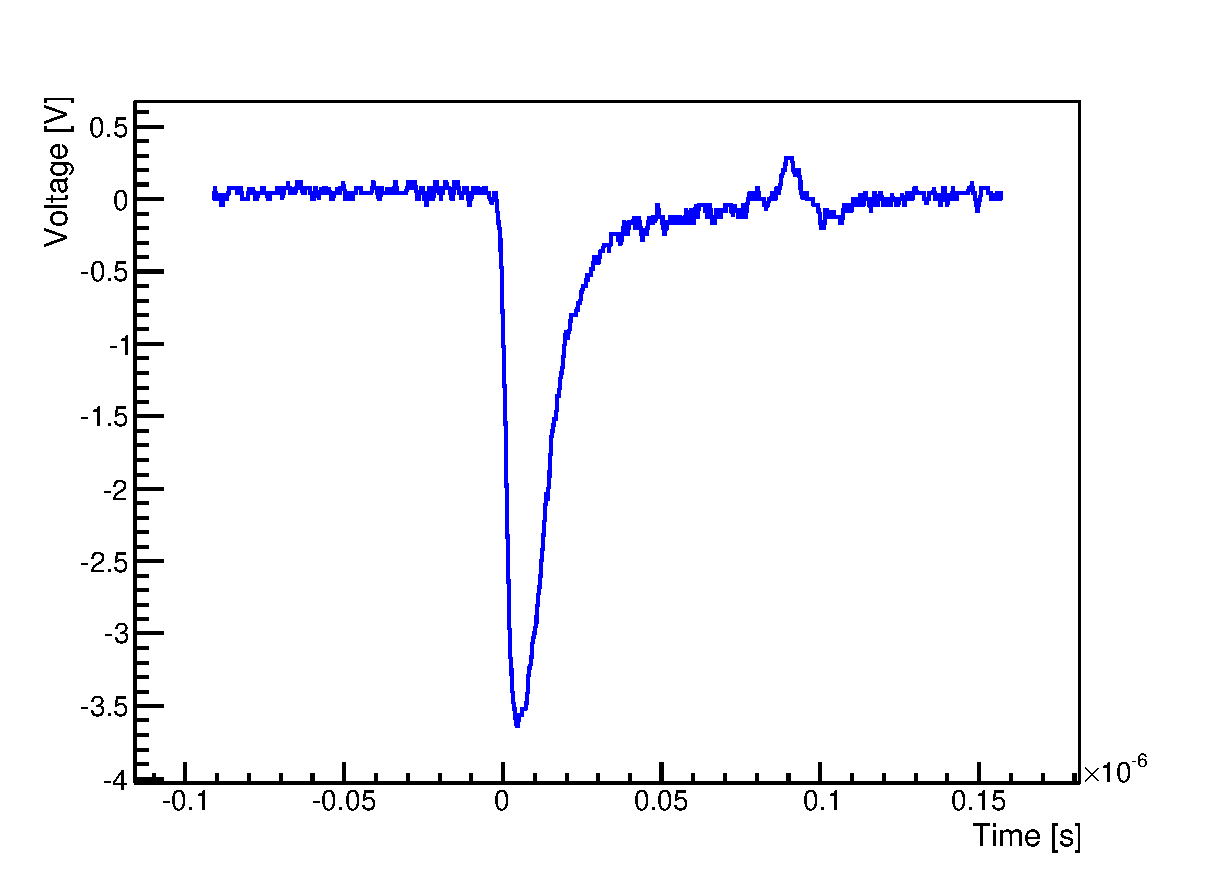
\includegraphics[width = 0.9\textwidth]{graphics/muonModules/monSpec/muonSignal.eps}
	\caption[Muon signal shape]{Pulser shape on the left compared to actual signal shape on the right. }
  \end{figure}
	\begin{figure}
	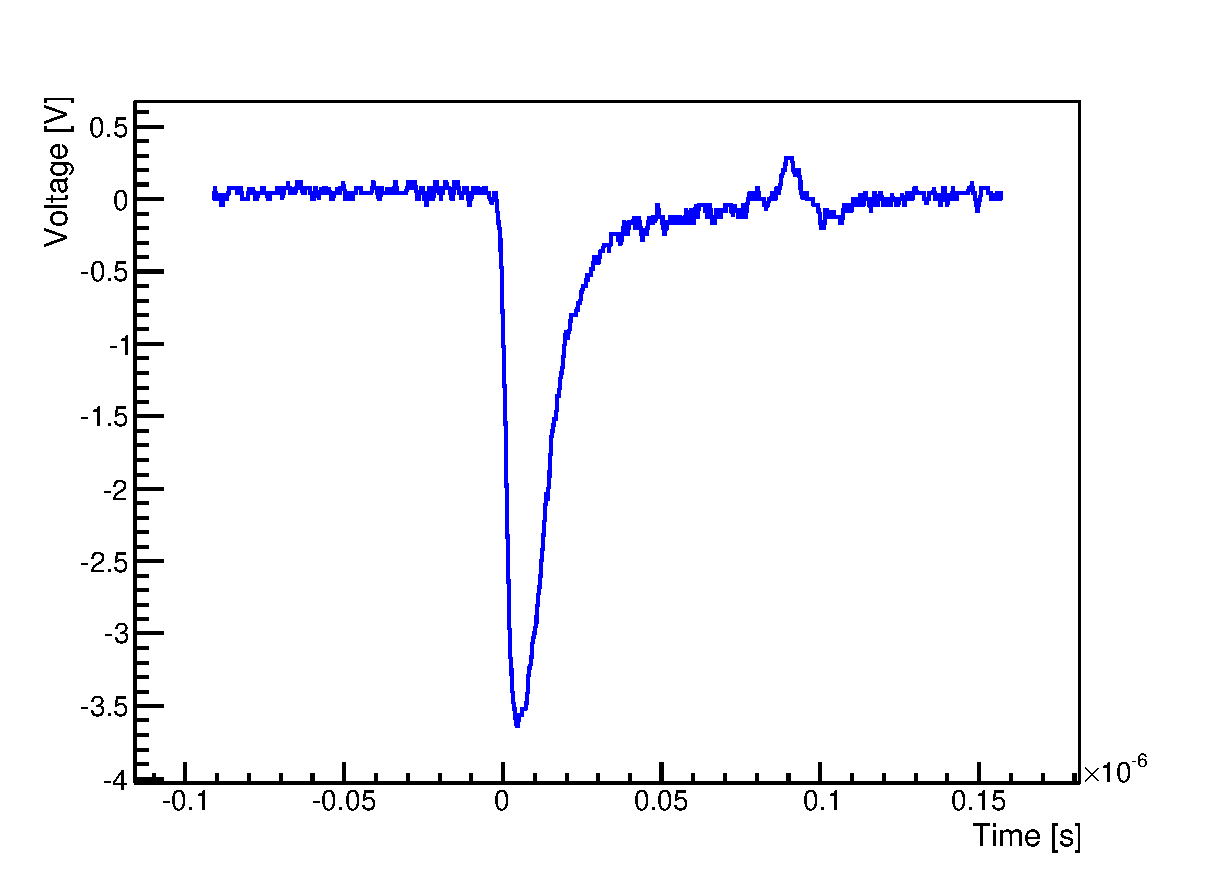
\includegraphics[width = 0.9\textwidth]{graphics/muonModules/monSpec/muonSignal.eps}
	\caption[Pulser and signal shape]{Pulser shape on the left compared to actual signal shape on the right. }
  \end{figure}
  
  In order to evaluate filter's figure of merit, the width of the resulting energy histogram, which should, assuming perfect pulser signals and perfect filters, be mono-energetic, was analyzed for each filter setting. For analysis, the width of the contributing ADC bins and their absolute position as well as the pulse height and the filter settings were noted. 
  
  \begin{table}
	\begin{tabular}{c}
	\SI{0}{\nano\second} gap, \SI{0}{\second} shaping time\\
	\end{tabular}
  	\begin{tabular}{|c|c|c|c|c|}
  		\hline
  		Voltage[V] & Boxcar length [ns] & width & position & threshold\\
  		\hline
  		\multirow{4}{*}{1} & 50 & 33 & 2160 & 2100\\
  		 & 100 & 37 & 2140 & 4200\\
  		 & 150 & 13 & 2140 & 6300\\
  		 & 200 & 10 & 2141 & 8400\\
  		 \hline
  		 \multirow{4}{*}{2} & 40 & 25 & 2160 & 2100\\
  		 & 100 & 78 & 2140 & 4200\\
  		 & 150 & 78 & 2140 & 6300\\
  		 & 200 & 77 & 2141 & 8400\\
  		 \hline
  		 \multirow{4}{*}{3} & 59 & 25 & 2160 & 2100\\
  		 & 100 & 113 & 2140 & 4200\\
  		 & 150 & 110 & 2140 & 6300\\
  		 & 200 & 112 & 2141 & 8400\\
  		 \hline
  		 \multirow{4}{*}{4} & 80 & 25 & 2160 & 2100\\
  		 & 100 & 145 & 2140 & 4200\\
  		 & 150 & 147 & 2140 & 6300\\
  		 & 200 & 149 & 2141 & 8400\\
  		 \hline
  		 \multirow{4}{*}{5} & 94 & 25 & 2160 & 2100\\
  		 & 100 & 180 & 2140 & 4200\\
  		 & 150 & 185 & 2140 & 6300\\
  		 & 200 & 41 & 2141 & 8400\\
  		 \hline	
  	\end{tabular}
  \caption[Energy resolution dependant on filter setting]{Energy resolution at different filter settings. A function generator was used to simulate pulses from the muon modules.}
	\centering
  \end{table}
  
  On average, the boxcar filter at shaping lengths of \SI{150}{\nano\second} shows the most promising results, i.e. the sharpest energy resolutions for any signal height. This concurs with the settings chosen for the active fpd veto; here slightly longer (around \SI{30}{\nano\second}) but comparable signals enter the DAQ's FLT cards showing best results at the same filter settings\cite{KevinWierman}.
  That is why, for any measurements after \todo{run \& date}, the new filter settings were used, bringing up the need for new threshold and gain adaptions \ref{ch:The muon detection system:sec:Gains, Thresholds and Acceleration Voltages}. 
  
  %% ===========================
  \section{Moun module's rates}
  \label{ch:Analysis:sec:Muon module's rates}
  %% ===========================  
  A simple first check into the data was possible simply by comparing the rates measured to literature values. Here, a flux of around 1 per \SI{}{\minute} and \SI{}{\square\centi\meter} through an area parallel to the ground is stated. Measured rates are in the order of \SI{250}{\hertz}. The muon modules' area is
  \begin{equation}
  	\SI{315}{\centi\meter} \cdot \SI{65}{\centi\meter} = \SI{2.05}{\square\meter}
  \end{equation}
  considering the \SI{45}{\degree} tilt of the modules towards the horizontal, this area reduces to an effective area of 
  \begin{equation}
  	A_{\mathrm{eff}} = \sin{\left(\SI{45}{\degree}\right)} A_{\mathrm{real}} = \SI{1.45}{\square\meter}
  \end{equation}
  Further taking into account detection efficiencies $\eta$ discussed in \ref{ch:Analysis:sec:Module Efficiency}, we receive an estimation of effective rate of
  \begin{equation}
  	\Phi_{est} = \eta \frac{1}{\SI{}{\square\centi\meter}\SI{60}{\second}}A_{\mathrm{eff}} = \SI{225}{\hertz}
  \end{equation}
  This compares well to measured rates of \todo{calculate actual rates} ~ \SI{250}{\hertz}.
  
  %% ===========================
  \section{Modules in high magnetic fields}
  \label{ch:Analysis:sec:Modules in high magnetic fields}
  %% ===========================  
  For there is the need of moving the muon modules as close to the spectrometer tank as possible to register mostly muons that indeed went through the vessel, they are aligned closely to the air coil system. This brought up the problem of photomultiplier tubes having to work in high magnetic fields. Photomultipliers, as mentioned before, use electrons cascading in electric fields to generate amplified signals. Additional magnetic fields can keep the electrons from reaching the dynodes stopping the cascade thus keeping single events from being registered. As rate decreases strongly under these conditions \todo{are there runs showing that? ask nancy}, a solution needed to be found. As a simple, yet efficient passive counter measurement, a layer of mu-metal was wrapped around the modules. Mu-metal is a magnetically highly permeable material (here, $\mu_r\approx $\todo{find out permeability}) that guides the magnetic field lines inside itself. In doing so, the remaining flux inside a mu-metal surrounded volume, 
and with it the field strengths, drastically reduces.
  To test the improvement the mu metal coverage produces, measurements with rising aircoil currents have been performed.
  Steps in the size of tenths of the maximum current of mostly \SI{100}{\ampere}, in some cases only \SI{70}{\ampere}, were used to record rates over half an hour at each value.
  During the first run, due to a slow control problem, the current was not raised between two steps. Although displaying the expected behavior - rates dropped much less than before - the measurement was repeated with the correct currents.
  Measurements show that the rate still drops at currents close to the maximum, though only to around \SI{90}{\percent} of initial values, see figure \ref{fig:aircoilCountsCurrent}. As, under normal measurement conditions, the coil currents are mostly around half the maximum value or less, the problem could be solved, as here, the reduction in rate is within the errors' order.
  \begin{figure}

  \centering
  	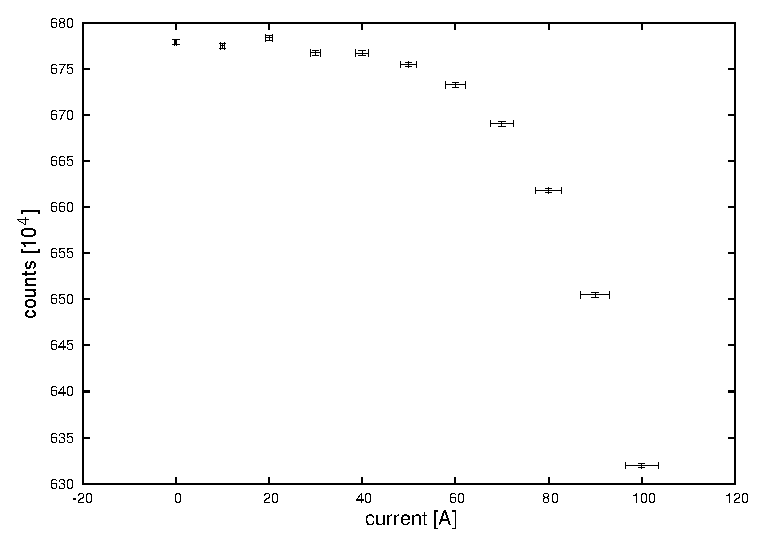
\includegraphics[width = 0.9 \textwidth]{graphics/aircoilCounts/aircoilsCountsCurrent.eps}
  	\caption[Rate dependence on magnetic fields]{Counts over air coil currents, with a maximum of \SI{100}{\ampere}. A clear decrease in rate is recognizable in the last 5 data points.}
  	\label{fig:aircoilCountsCurrent}
  \end{figure}
  

  %% ===========================
  \section{Module Stability}
  \label{ch:Analysis:sec:Module Stability}
  %% ===========================  
  If consistent factual statements on muon induced background are to be made, the modules need to work stable over the course of days, as rates are supposed to be comparable. For this reason, over the Christmas time 2012, a two-weekly measurement of half hourly runs was taken, see table \ref{tab:airCoilSettingsChristmas} for air coil settings used. Runs myo00000051 to myo00000675 contain the data of this measurement.
  \begin{table}
  \centering
   \begin{tabular}{|l|ccccccc|c|}
    \hline
    &&&&&&&&\\
    Coil \#	&1	&2	&3	&4	&5	&6	&7	&EMCS h	\\
    Current [A]	&10	&10	&14	&25	&42	&39	&54	&50  	\\
    &&&&&&&&\\
    Coil \# 	&8	&9	&10	&11	&12	&13	&14	&EMCS v	\\
    Current [A]	&54	&21	&36	&30	&21	&20	&56	&15    	\\
    &&&&&&&&\\
    \hline
   \end{tabular}
  \caption[LFCS settings stability measurement]{Runtime settings for air coils as proposed and for the commissioning measurements. These were kept static over the two weeks end 2012/beginning 2013}
  \label{tab:airCoilSettingsChristmas}
  \end{table}
  The time slot was chosen for the lowly frequented spectrometer hall's sake to minimize external impacts on data taking. For analysis, a simple program to count events in variable time bins was written, creating a count histogram for all the runs in the measurement period. The result can be seen in figure \ref{fig:moduleStability}. The observable fluctuation is well describable by fluctuations in atmospheric density, i.e. pressure $\Delta p$ and temperature $\Delta T$ and in muon production height $\Delta h$\cite{muonIntensity}.
  \begin{equation}
  	\frac{\Delta I}{I} = - (\alpha_\mu\Delta p + \beta \Delta h -\gamma \Delta T)
  \end{equation}
  where $\alpha$ is a barometric coefficient in \SI{0.215}{\percent\per\mmHg}, $\beta$ a decay coefficient in \SI{5}{\percent}/\SI{10e3}{\meter} and $\gamma$ a temperature coefficient in \SI{0.1}{\percent\per\kelvin}
  If one looks at the data from \cite{wetterCom} the fluctuations, only available on a daily basis, are comparable to the ones visible in the data of the stability measurements. To make graphs more comparable, the data has been analyzed again, now with daily binning. It has to be kept in mind that the weather data was obtained from a weather station in Rheinstetten, about \SI{20}{\kilo\meter} from KIT campus north, and represents only the lowest atmospheric layer while muons are generated mostly in the upper layers of the atmosphere.
  \begin{figure}
	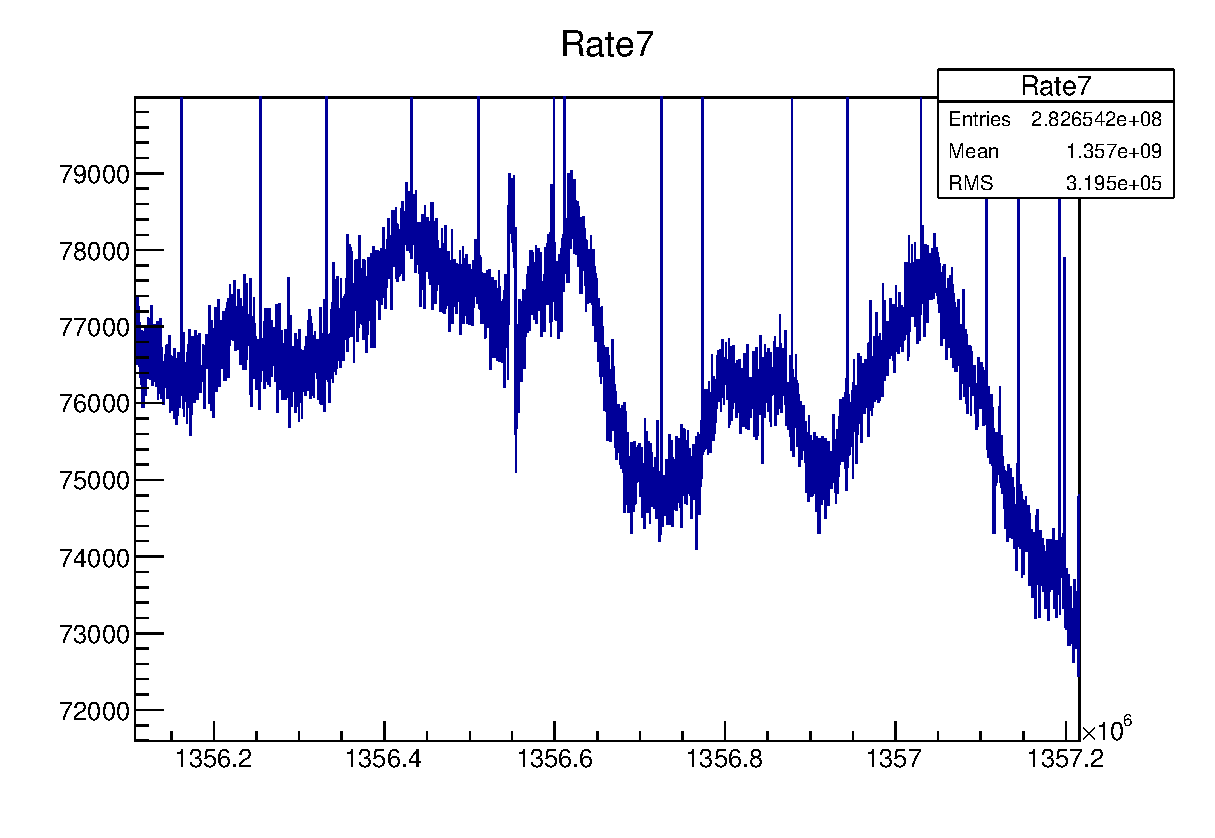
\includegraphics[width = 0.9 \textwidth]{graphics/setup/stability.eps}
  	\caption[Muon module stability]{Rate per five minutes over the course of about two weeks (21-12-2012 to 03-01-2013). }
  \end{figure}

  \begin{figure}
	\centering
  	\includegraphics[width = 0.9 \textwidth]{graphics/dummy.eps}
  	\caption[Atmospheric density stability measurement]{Atmospheric density as a function of time over the course of two weeks the muon measurements took place. Note the }
  	\label{fig:moduleStability}
  \end{figure}

  %% ===========================
  \section{Module Efficiency}
  \label{ch:Analysis:sec:Module Efficiency}
  %% ===========================  
  The runs used for stability measurements, as well as any other run including modules six, seven and eight, can be used to check muon module seven for efficiency. For tests on other modules, the geometry would need to be changed so that the one to be checked is in between at least two other modules.
  For analysis, the function determineEfficiency() \ref{ch:Analysis software:sec:methods of the class run:subsec:determineEfficiency}
  has been written.
  The principle is the following: considering the small change in momentum direction high energy muons achieve through interaction with matter, one can assume straight-lined paths. From that follows, that if two parallel planes, that can be used to describe the scintillating volumes, are hit, any other, also parallel plane, in between those two will be hit as well. Keeping this in mind, one can analyse data for events registered in both modules 6 and 8 and cross check whether a event has been detected in module 7 as well. The quota of events in all three modules compared to those detected in 6 and 8 -  including the triple events - shows the efficiency of module 7.
  It shows that during the measurement period end of 2012, the efficiencies were at \todo{rerun} \SI{94 }{\percent} which is less than one would expect at a scintillator thickness of \SI{5}{\centi\meter} for muons perpendicular to the largest module surface, even more for any other.
  For that reason, the filter settings were checked and changed to the boxcar filter with a gap of \SI{150}{\ns} from the before used \todo{exact name} filter. However, the expected efficiency increase was not observable, the average efficiencies before and after are within the margin of error of the other.
  To examine the problem further modules 3, 4 and 5, that are located next to each other, were used for efficiency measurements as well considering they are stacked in an upright way. Using the program on those three modules resulted in even lower efficiencies of \SI{50(3)}{\percent}. This raises the question whether this is not an effect of signal filtering, but a previously not considered physics effect. One thing coming to mind is deviation of the muon track from linear forms. This feature would comply with the seemingly lower efficiency at the upright stacked modules, where, at equal bending radii, the ratio of muons traveling around the middle module is higher due to the lower total area in stacking direction.
  This thesis should be tested. This can be done both by simulating the cosmic muons including magnetic fields and empirically by varying the distance between the single modules. The latter is difficult not only because the modules are heavy and not made for lifting (no designated carrying structures), but also because movement always means potential danger to the photomultiplier tubes and their connection to the scintillators.
  Furthermore, if all coils and solenoids were to be turned off simultaneously at some point, one could collect data then and see how efficiencies change during that (there have been runs taken when that was still the case, but only few modules were working properly at that point).
  If the dependence on module distance turns out to be true, but the efficiencies are still below expected values at the lowest possible distances, a possible improvement would be to use pre-amplifiers before signals arrive at the DAQ. These would widen the signals timewise leading to a more easily detectable signal for the filters.
  
  %% ===========================
  \section{Photo Multiplier Tube Test with Sr source}
  \label{ch:Analysis:sec:PhotoMultiplierTests}
  %% ===========================
  
  With sets of four photomultiplier tubes being read out over one cable, and, consequently, via one channel, the test of individual PMTs is not trivial. Nevertheless, a method using a \SI{}{\mega\becquerel} $\rm ^{90}Sr$ source to trigger events was used to check functionality. Of course, all tubes were able to see the source at any position but rates were expected to rise as the distance to any of the tubes shrank. A source holder was constructed from acrylic glass to shield the user from radiation and to attach the source to the modules, as a large dependence of rate on the position was found when the source was simply duct taped to the modules. As the foil mantling of the modules absorbs a non negligible part of the radiation emitted from the source, it had to be ensured that the number of layers was equal for all measurements. This was given only below the modules as the foil has been folded around them at the ends in a gift wrapping way. Thus, the source was pretty far away from the photomultiplier tubes making it more difficult to distinguish between them. A first measurement was to check for exactly this distinguishability.
  
  \begin{figure}
%   	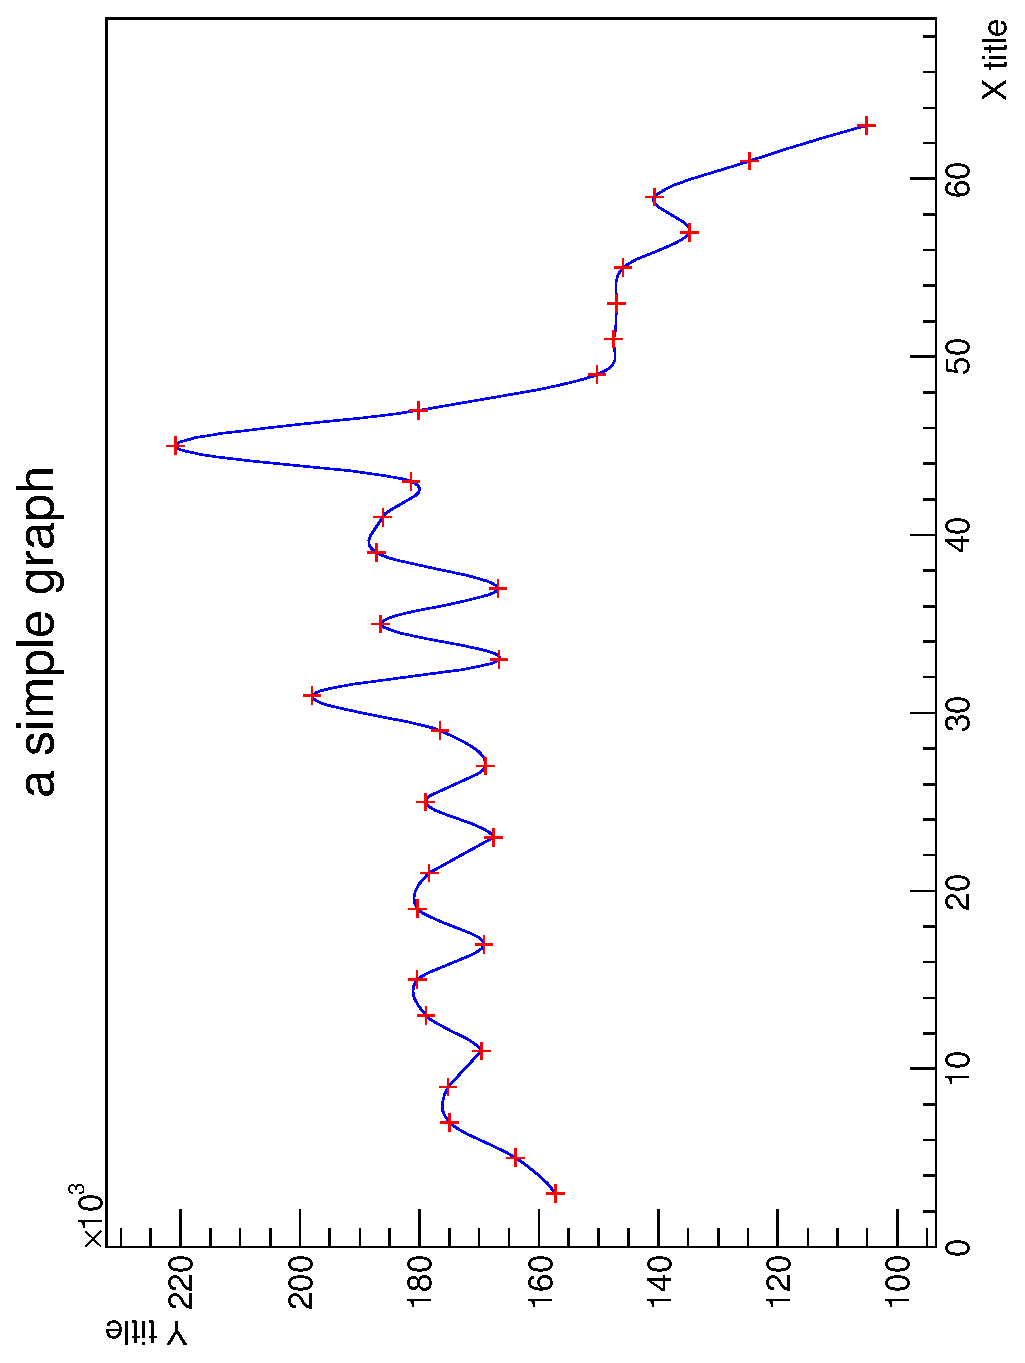
\includegraphics[angle = -90, width = 0.9 \textwidth]{graphics/cobalt/874_parallel_2cm_steps.ps}
  	\caption[Rate scanning with cobalt source]{}
  \end{figure}

  \begin{figure}
  \centering
%   	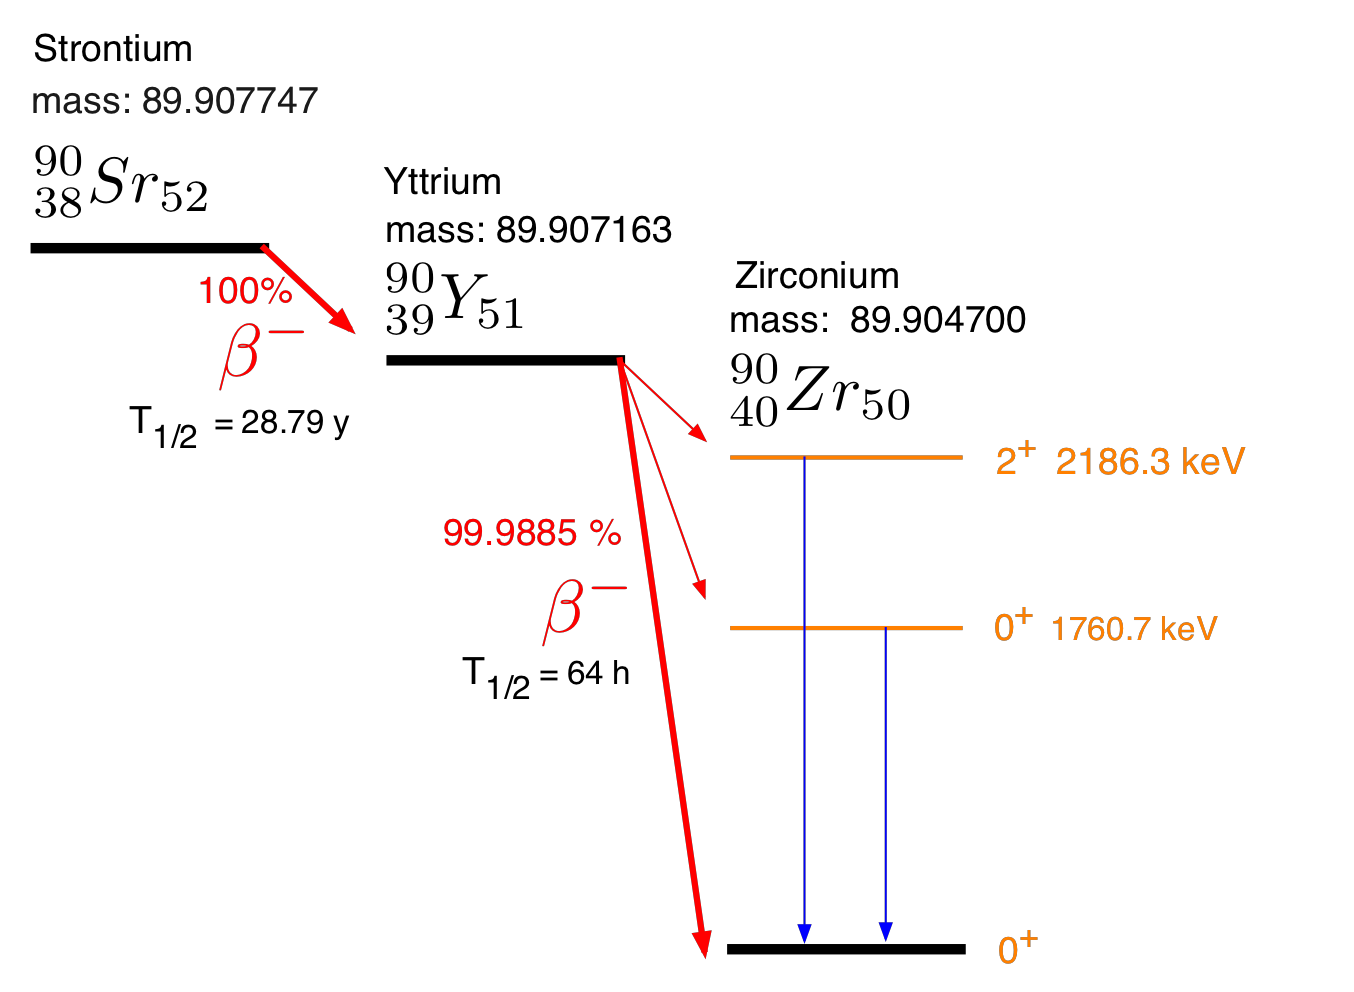
\includegraphics[width = 0.5 \textwidth]{graphics/cobalt/Sr90_decay.eps}
  	\caption[Cobalt decay scheme]{Decay scheme of $^{90}$Sr: first a lower energetic decay to $^{90}$Y emitting \SI{544}{\kilo\electronvolt}/\SI{}{\square c} electrons, from that most probably a higher energetic decay to $^{90}$Zr ground state (\SI{2.29}{\mega\electronvolt}/\SI{}{\square c} electrons) or, with low probabilty, to one of two of its excited states.}
  \end{figure}

  As one can see a rise in rate at the positions the tubes are located at, it was decided that four measurements per module and side were sufficient, especially as all measurements can afterwards be compared to each other.
  The tube positions at \todo{n,n,n,n cm} were used as measurement positions as well. For each side, a run has been taken containing five minute subruns for every position. Figure \ref{fig:SrRatesPMT12} to \ref{fig:SrRatesPMT678} show the result of these measurements. One can see that the gerneral shape of each side compares very well to the others. Exceptions are \todo{which ones different?}showing slight, but acceptable deviations off the norm.
  \begin{figure}
		\centering
		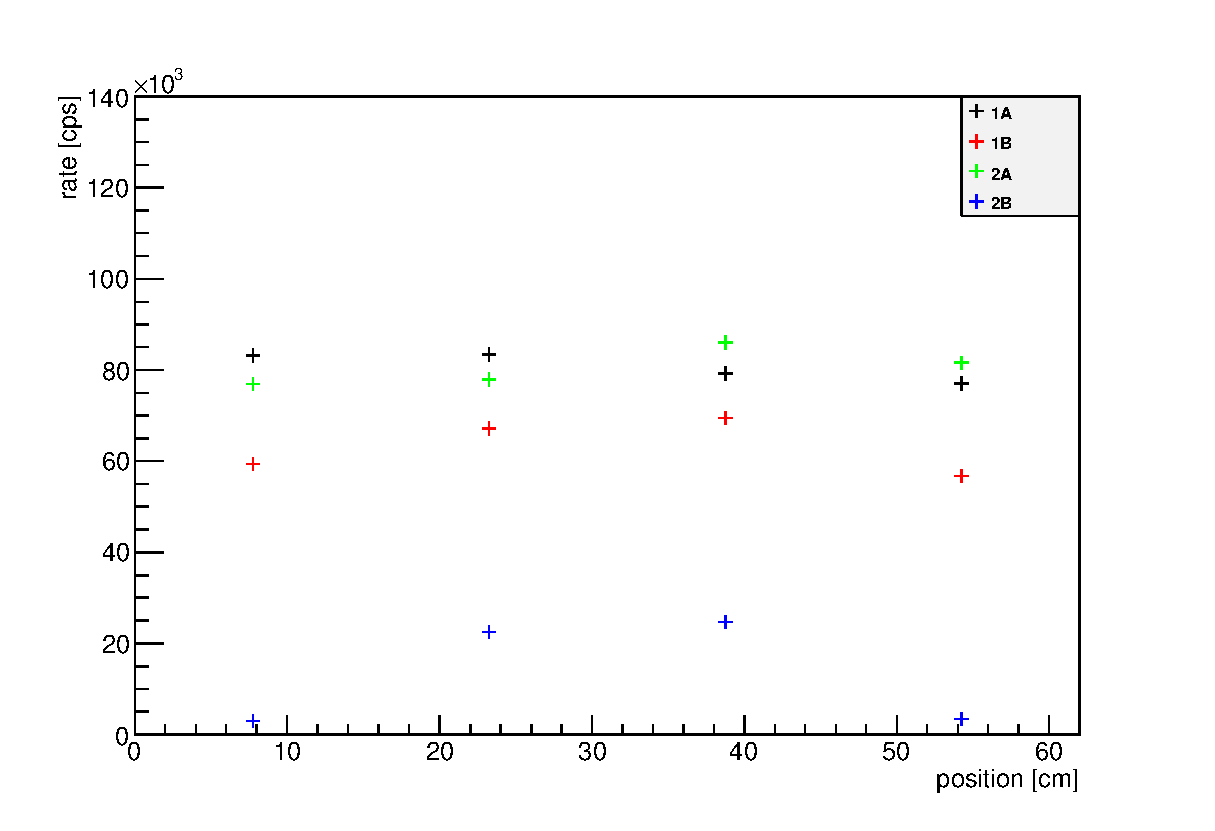
\includegraphics[width = 0.9\textwidth]{graphics/analysis/12final.eps}
  	\caption[Testing of muon modules with Sr source - Modules 1 \& 2]{Measurements with the source at four different positions. Both sides of modules 1 and 2. Noticable are the much lower rates for module 2B which is one of the two that was later set to \SI{1.6}{\kilo\volt} acceleration voltage. }
  	\label{fig:SrRatesPMT12}
  \end{figure}
    \begin{figure}
		\centering
		\includegraphics[width = 0.9\textwidth]{graphics/analysis/345final.eps}
  	\caption[Testing of muon modules with Sr source - Modules 3 - 5]{Measurements with the source at four different positions. Both sides of modules 3 to 5 are shown. Except for single measurement points that are standing out, the different sides show similar rates. }
  	\label{fig:SrRatesPMT12}
  \end{figure}
    \begin{figure}
		\centering
		\includegraphics[width = 0.9\textwidth]{graphics/analysis/678final.eps}
  	\caption[Testing of muon modules with Sr source - Modules 6 - 8]{Measurements with the source at four different positions. Both sides of modules 6 to 8. Noticable are the lower rates for module 6B which again is one of the two that was later set to \SI{1.6}{\kilo\volt} acceleration voltage. }
  	\label{fig:SrRatesPMT12}
  \end{figure}

    %% ===========================
  \section{Synchronisation of moun module and FPD DAQs}
  \label{ch:Analysis:sec:Synchronisation of moun module and FPD DAQs}
  %% ===========================  
  Measuring time differences between detector signals and muon events on a \SI{}{\micro\second} scale requires exact synchronization of the two different DAQs. For this purpose, a clock has been designed sending signals at two frequencies: one at \SI{1}{\hertz} and one at \SI{10e6}{\hertz} internally converted to a \SI{20 e 6}{\hertz} signal by the DAQ. Those signals can be synchronized to the timestamps of GPS satellites if a GPS antenna is connected. This has not yet been done as relative synchronization between the two crates is sufficient for the purposes of finding correlations between muon and detector events. As the cable length for signal transmission is pretty extensive - around \SI{50}{\meter} - it was decided to use optical fibers instead of CAT 5 cabling. As two signals need to be transmitted, paired \todo{connection type name} fibers were used. The clock itself has optical outputs, the DAQ though needs converters from optical to electrical signals and a modified SLT back panel card to receive the converted 
signals via Cat5 cabling.
  \begin{figure}
  	\includegraphics[width = 0.9 \textwidth]{graphics/dummy.eps}
%   	\includegraphics[width = 0.9 \textwidth]{graphics/sync/GPSclock.jpg}
  	\caption[Unsynced DAQs]{With the old firmware installed, one can see a difference of $\approx$ \SI{}{\micro\second} between events recorded. As the signals occur simultaneously and the DAQs are synchronised, this difference should vanish.}
  	\label{fig:analysis:outOfSync}
  \end{figure}

  
  To test the setup, the muon DAQ was moved to the detector platform. Both crates were fed by a pulser signal. Runs at different frequencies were recorded to test both the synchronization and the detection of events. To synchronize timestamps to an external signal, the FLT cards drop down menu needs to be set to \todo{look up} and the SLT needs to be set to \todo{lookup too}.
  At first, manually triggered signals were used in minute runs to check the timestamps equality. Several runs were taken, all showing that the events were shifted by several \SI{}{\micro\second}.
  \begin{figure}
	\includegraphics[width = 0.9 \textwidth]{graphics/dummy.eps}
% 	\includegraphics[width = 0.9 \textwidth]{graphics/sync/nonSynced.eps}
  	\caption[Unsynced DAQs]{With the old firmware installed, one can see a difference of $\approx$ \SI{}{\micro\second} between events recorded. As the signals occur simultaneously and the DAQs are synchronised, this difference should vanish.}
  	\label{fig:analysis:inSync}
  \end{figure}

  In close cooperation with the IPE it was found that this was merely a problem of firmware versioning as well as software settings in ORCA resolving the problem quickly. After installing the latest firmware, more runs were taken now displaying the desired behavior:
  \begin{figure}
	\caption[Synchronisation new firmware]{Time differences between events after firmware upgrades. Differences between the event times are within one \SI{50}{\nano\second} bin}
	\includegraphics[width = 0.9 \textwidth]{graphics/dummy.eps}
	%   	\includegraphics[width = 0.9 \textwidth]{graphics/sync/synced.eps}
  \end{figure}
  Following the manually triggered events, runs with fixed frequency events were recorded, raising the frequency to up to \SI{10}{\kilo\hertz}. Doing so, different recording modes and filter settings were applied - see table \ref{tab:syncTests}. All the tests worked fine including starting one DAQ's run way ahead of the other. Those events recorded in both run files were always well synchronized.
  \begin{table}
  \centering
  	\begin{tabularx}{0.9 \textwidth}{|X|cc|}
  	\hline
  		\bf{Settings} & \bf{fpd run} & \bf{myo run}\\	
  		\hline
  		\multicolumn{3}{|c|}{Pulser voltage 250mV, freq (sampling) 100000, waveform: needle negative}\\
  		\hline
		as before, but 300sec runs & 4174 & 710 \\
		as before, but 300sec runs and energy+trace mode (sync) & 4175 & 711 \\
		5 random pulses within 60sec run & 4176 & 712 \\
		pulser frequency: 1 Hz, 60sec run & 4177 & 713 \\
		pulser frequency: 10 Hz, 60sec run & 4178 & 714 \\
		pulser frequency: 100 Hz, 60sec run & 4180 & 715 \\
		pulser frequency: 1 kHz, 60sec run & 4181 & 716 \\
		pulser frequency: 10 kHz, 60sec run & 4182 & 717 \\
		Pulser:&&\\
		\hline
		\multicolumn{3}{|c|}{Pulser voltage 150mV, Freq (sampling) 1000, waveform: Pin diode negative}\\
		\hline
		5 random pulses within 60sec run & 4184 & 719 \\
		increased thresholds from 500 to 1000 (both)
		pulser frequency: 1 Hz, 60sec run & 4185 & 720 \\
		pulser frequency: 10 Hz, 60sec run & 4186 & 721 \\
		pulser frequency: 10 Hz, 300sec run & 4187 & 722 \\
		pulser frequency: 100 Hz, 300sec run & 4188 & 723 \\
		pulser frequency: 10 Hz, 300sec run & 4189 & 724 \\
		\hline
		\multicolumn{3}{|c|}{ Removing Cat5 cables from synchronization clock and }\\
		\multicolumn{3}{|c|}{ installing fiber optic cables + converter boxes}\\
		
		\hline
		pulser frequency: 0.2 Hz, 60sec run & 4190 & 725 \\
		5 random pulses within 60sec run, both energy mode & 4191 & 726 \\
		pulser frequency: 1 Hz, both energy mode, 60sec run & 4192 & 727 \\
		pulser frequency: 10 Hz, both energy mode, 60sec run & 4193 & 728 \\
		pulser frequency: 10 Hz, both energy mode, 300sec run & 4194 & 729 \\
		pulser frequency: 100 Hz, both energy mode, 300sec run & 4195 & 730 \\
		pulser frequency: 10 Hz, both energy+trace (sync) mode, 300sec run & 4196 & 731 \\
  		\hline
  	\end{tabularx}
	\caption[Synchronization test Settings]{All settings including run numbers tested with the two DAQs from detector system and muon modules. In the leftmost column, pulser settings and run lengths are described. In front of the different parts the pulser settings kept constant for the following measurements are described.}
	\label{tab:syncTests}
  \end{table}

  Afterwards, the muon DAQ was moved back to its original position and the optical fibers were stowed in wire-ways guiding it from the detector platform down to the basement where the muon detection system is located. Another problem occurred here, as signal transmission was impaired by a kink at one of the turns, but was quickly resolved by smooth rewiring.
  Concluding, it can be said that the clock runs continuously without any problems throughout all the measurements - including main spectrometer commissioning measurements.

  
  %% ===========================
  \section{Coincidence Search between Muon- and Detector Events}
  \label{ch:Analysis:sec:Monitor Spectrometer Measurements}
  %% ===========================  
  If one wants to actually detect background induced by muonic events detected by the muon modules, those events need to be correlated to detector events time wise. For this purpose, the analysis code's class run was extended by the member functions TOFHist()\ref{ch:Analysis software:sec:methods of the class run:subsec:TOFHist()} and TOFMuonDet()\ref{ch:Analysis software:sec:methods of the class run:subsec:TOFMuonDet()}, where the former is used for monitor spectrometer analysis and the latter for the main spectrometer. The biggest difference is that, for the main spectrometer, runs by two DAQs leading to different starting times and different lengths are created that need to be compared. Here, the necessity for synchronization from chapter \ref{ch:Analysis:sec:Synchronisation of moun module and FPD DAQs} becomes clear.
  
  %% =========================
  \subsection{Monitor Spectrometer}
  \label{ch:Analysis:sec:Monitor Spectrometer Measurements:subsec:Monitor Spectrometer}
  %% =========================
  
  Measurements at the monitor spectrometer are easily manageable due to the fast accessibility of all the components and the collection of data in a single run-file through the mini-crate.
  For measurements, high voltage supplies have been added to the \todo{name of the rack} rack and the readout electronics were connected to a second FLT-card inserted into the mini-DAQ and operated in veto-mode. Gains and thresholds were easily set as only four sides had to be adjusted - compared to the 16 main spectrometer channels. The PMT tubes were operated at \SI{1.5}{\kilo\volt}. The detector gain and threshold settings for the 5 pixel detector have been kept, although the detector position was shifted to the position at which the center pixel exhibited maximum rate and the pairs of east-west and top-bottom pixels showed comparable count rates. Furthermore, the recording mode was switched from histogram-mode to energy-mode as the timestamps for every single event were needed for analysis. 
  Several hourly runs were taken under different magnetic field compositions. Both asymmetric magnetic field (see table \ref{tab:analysis:asymmetricMagneticFields} and figure \ref{fig:monSpec:asymmetric magnetic field} and non-axially-symmetric field (see table \ref{tab:analysis:nonAxiallySymmetricField} and figure \ref{fig:monSpec:non axially symmetric magnetic field} configurations were investigated.
  \begin{table}
	\centering
		\begin{tabular}{c}
		\end{tabular}\\
		\begin{tabular}{|l|l|ccccccc|}
			\hline
			\centering
			
			Measurement &Run &  solenoid &solenoid &inner & outer &outer &emcs x	&emcs y\\
			& 	& source	& detector & aircoil & central aircoil & aircoil& &\\
			\hline
			A & mos00159395& 0&	25&	0&	-4&	-4&	2&	-19.5\\
			\hline
			 B & mos00159396-&&&&&&&\\
			& mos00159398 & 0 & 50& 0 & -8 & -8 & 2 & -19.5\\
			\hline
			C & mos00159399 & 0 & 50& 0 & -7 & -7 & 2 & -19.5\\
			\hline
			D & mos00159400 & 0 & 50& 0 & -6 & -6 & 2 & -19.5\\
			\hline
			E & mos00159401 & 0 & 10& 0 & -2 & -2 & 2 & -19.5\\
			\hline
			F & mos00160713-&&&&&&&\\
			& mos00160717& 0.1 & 12.5 & 0 & -2 & -2 & 0 & 0\\
			\hline
			G & mos00160718-&&&&&&&\\
			& mos00160730 & 0.1 & 12.5 & 0 & -2 & -2 & 0 & 0\\
			\hline
			H &mos00161105-&&&&&&&\\
			& mos00161107 & 0.1 & 12.5 & 0 & -2 & -2 & 0 & 0\\
			\hline
			I &mos00161108-&&&&&&&\\
			 & mos00161110 & 0.1 & 25 & 0 & -2 & -2 & 0 & 0\\
			\hline
		\end{tabular}
		\caption[Asymmetric magnetic field measurements]{Measurements at asymmetric magnetic fields. The source side magnet was turned off for all measurements leaving the flux tube entering the spectrometer walls.}
		\label{tab:analysis:asymmetricMagneticFields}
	\end{table}
	\begin{table}
		\begin{tabularx}{\textwidth}{|L{1.1cm}|>{\centering}X|>{\centering}X>{\centering}X>{\centering}X>{\centering}X>{\centering}X>{\centering}X>{\centering\arraybackslash}X|}
			\hline
			\parbox[t]{2mm}{\multirow{3}{*}{\rotatebox[origin=c]{90}{ Run mos00... }}}
			&\parbox[t]{2mm}{\multirow{3}{*}{\rotatebox[origin=c]{90}{\bf 2 Horizontal loops }}}
			&\parbox[t]{2mm}{\multirow{3}{*}{\rotatebox[origin=c]{90}{solenoid source }}}
			&\parbox[t]{2mm}{\multirow{3}{*}{\rotatebox[origin=c]{90}{solenoid detector }}}
			&\parbox[t]{2mm}{\multirow{3}{*}{\rotatebox[origin=c]{90}{inner aircoil }}}
			&\parbox[t]{2mm}{\multirow{3}{*}{\rotatebox[origin=c]{90}{ outer aircoil }}} 
			&\parbox[t]{2mm}{\multirow{3}{*}{\rotatebox[origin=c]{90}{outer cent. aircoil }}}
			&\parbox[t]{2mm}{\multirow{3}{*}{\rotatebox[origin=c]{90}{EMCS x }}}
			&\parbox[t]{2mm}{\multirow{3}{*}{\rotatebox[origin=c]{90}{EMCS y }}}\\
			
			
			
			&&&&&&&&\\
			&&&&&&&&\\
			&&&&&&&&\\
			&&&&&&&&\\
			&&&&&&&&\\
			&&&&&&&&\\
			&&&&&&&&\\
			\hline
			161111-161125 & 0 & 25 & 25 & 6.8 & -7 & 5 & 0 & -14\\
			\hline
			161126-161129 & +50 & 12.5 & 12.5 & 3.5 & -3.5 & 2.5 & 0 & 0\\
			\hline
			161130-161133 & +25 & 12.5 & 12.5 & 1.75 & -1.75 & 1.25 & 0 & 0\\
			\hline
			161134-161149 & -25 & 12.5 & 12.5 & 1.75 & -1.75 & 1.25 & 0 & 0\\
			\hline
			161150-161155 & -50 & 12.5 & 12.5 & 3.5 & -3.5 & 2.5 & 0 & 0\\
			\hline
			161156-161158 & 0 & 12.5 & 12.5 & 3.5 & -3.5 & 2.5 & 0 & 0\\
			\hline

			
			\hline
		\end{tabularx}
		\caption[Non axially-symmetric magnetic field measurements]{Measurements in energy mode at non axially symmetric magnetic field. Both solenoid and air coil currents have bee changed, though always by a multiplication factor for all of them so that the ration remained the same.}
		\label{tab:analysis:nonAxiallySymmetricField}
		
  	\end{table}
  	
  	
  The TOFHist function (chapter \ref{ch:Analysis software:sec:methods of the class run:subsec:TOFHist()}) has been used to analyze the data.
  It browses through all the muon-events detected and finds any detector event in a definable timespan after the muon-event. This can be more than one detector-event per  muon-event. In all of the settings, a clear peak is visible at around \SI{7}{\micro\second}. As for count rates, they are a lot higher in the asymmetric magnetic field setup as secondary electrons are guided from their point of origin to the detector instead of mostly being magnetically shielded. In this setup, only the reflection through the rise in magnetic field on the electrons' paths takes its toll on the rate.
  A graphic of the flux tube configuration as well as the histograms for all of the settings can be found in the \ref{appendix}, figures \todo{reference figures.}
  The exact values are:
  \begin{table}
  	\begin{tabularx}{0.8\textwidth}{>{\centering}X>{\centering\arraybackslash}X}
  		Average & Standard Deviation\\
  	\end{tabularx}
  \end{table}

  \todo{Do analysis for every measurement, insert peak positions + stdev}
  
  
  \begin{figure}
	\includegraphics{graphics/dummy.eps}
	\caption[Asymmetric magnetic field flux tube]{Flux tube at asymmetric magnetic fields. Electrons from processes at the walls are guided directly towards the detector as the largest part of the flux tubes surface ends in the monitor spectrometer's vessel's wall}
  	\label{fig:monSpec:asymmetric magnetic field}
  \end{figure}

    \begin{figure}
	
	\includegraphics{graphics/dummy.eps}
  	\caption[Non-axially symmetric magnetic flux tube]{Flux tube at non axially symmetric fields. Although no direct guidance from the wall to the detector is given (the flux tube never touches the wall in this configuration), by adding a magnetic component perpendicular to z-direction, the probability for entrance into the flux tube rises strongly.}
  	\label{fig:monSpec:non axially symmetric magnetic field}
  \end{figure}
  
  \begin{figure}
	\label{fig:monSpec:timeDifferences asymmetric magnetic field}
	\caption[Time difference histogram]{Time difference histogram for asymmetric magnetic fields.}
  	\includegraphics{graphics/dummy.eps}
  \end{figure}
  
  \begin{figure}
	\label{fig:monSpec:timeDifferences non axially symmetric magnetic field}
	\caption[Non-axially symmetric magnetic flux tube monitor spectrometer]{Flux tube at non axially symmetric fields. Although no direct guidance from the wall to the detector is given (the flux tube never touches the wall in this configuration), by adding a magnetic component perpendicular to z-direction, the probability for entrance into the flux tube rises strongly.}
  	\includegraphics{graphics/dummy.eps}
  \end{figure}  
  %% =========================
  \subsection{Main Spectrometer}
  \label{ch:Analysis:sec:Monitor Spectrometer Measurements:subsec:Main Spectrometer}
  %% =========================
  
  Monitor-spectrometer results suggested that the time of flight was well measurable, even if on bigger scale, at the main spectrometer. So, during commissioning measurements, already parallel to first measurements ``M1'', some runs with asymmetric magnetic field have been taken with switched polarity or turned off pre spectrometer magnets compared to standard setup.
  The data was analysed for each single ring of the FPD. Search parameters were the time slot from \SI{0}{\second} to \SI{15}{\micro\second} though remains inconclusive at the moment, see \ref{fig:mainSpec:allRings}. Analysis for every single pixel was not possible due to far too low statistics, though it might be more conclusive as less different paths contribute to a single pixel. On the other hand, after the non-central alignment of the detetor has been fixed using different settings for the LFCS-system, under asymmetric magnetic fields, the fields should be rotationally symmetric around the z-axis disregarding small deviations. Assuming this, the path lengths for every pixel of one ring should be very comparable.
  
  \begin{figure}
  \centering
  	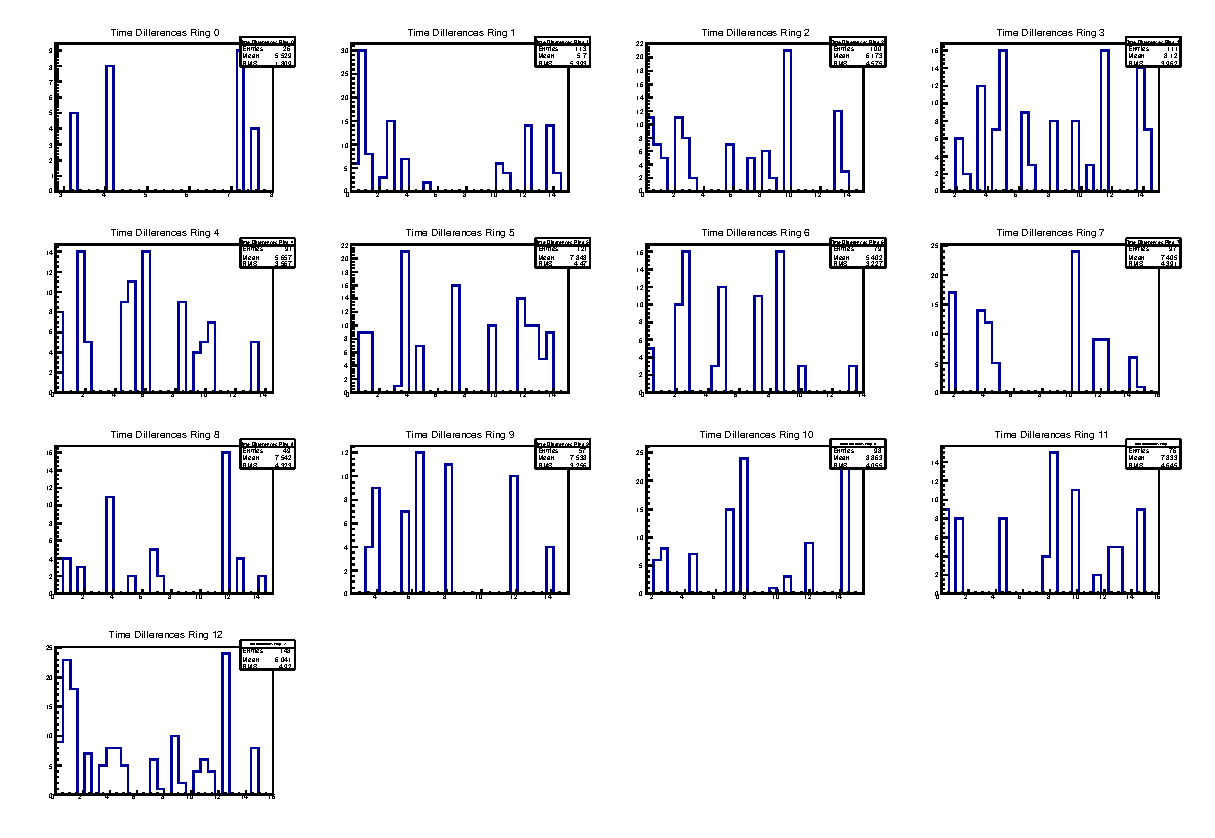
\includegraphics[width = 0.9 \textwidth]{graphics/mainSpec/mainSpecRings.eps}
  	\caption[Time difference Histogram for all rings]{Time differences of muon events followed by a detector event. From left to right and top down for every single detector ring, 0 being the innermost and 12 being the outermost ring. No clear indication of a time of flight for electrons induced by muons visible.}
  	\label{fig:mainSpec:allRings}
  \end{figure}

  
  The failure to find a clear runtime for electrons induced by muonic events might be due to the combination of muon module position and the magnetic field setup as the wall area covered by the flux tubes and the volume surveilled by the muon modules did not overlap very much. Furthermore, due to the very low magnetic field at the wall compared to the volume inside the detector and pinch magnet, most of the induced electrons are magnetically reflected as the maximum polar angle towards magnetic field lines $\theta_{max}$ is defined by
  \begin{equation}
  	\frac{B_{min}}{B_{max}} \approx \frac{\SI{3}{\gauss}}{\SI{4}{\tesla}} = sin^2(\theta_{max})
  \end{equation}
  meaning only angles satisfying the inequation
  \begin{equation}
  	\theta < \arcsin{\sqrt{\frac{B_{min}}{B_{max}}}} = \arcsin{\sqrt{\frac{\SI{3}{\gauss}}{\SI{4}{\tesla}}}} = \SI{0.004}{\degree}
  \end{equation}
	will be able to reach the detector. All others will be reflected and fly back to the wall to be absorbed in the conducting wall material. \todo{set real field values}
	As a result, compared to the monitor spectrometer, where the ratio is a lot greater, less of the muon induced electrons arrive at the detector making long measurements a requirement for good statistics. This leads to detector rates of only around \SI{2}{\cps}, depending on the inner electrode voltages.
	At high inner electrode voltages, the rate increases strongly to \SI{150}{\cps} which is probably due to field emission from the electrodes. Here, the rate of events actually analysed can be reduced by using energy cuts and excluding pixels with either known problems - for example the two defective pixels - or such covered by the misaligned flapper valve. The relevant energies were \SI{25.6}{\kilo\electronvolt} to \SI{30.6}{\kilo\electronvolt} including the PAE voltage of \todo{add PAE voltage}.
	To raise the overall acceptance of the muon induced events, these measurements were repeated with the main vessel on high voltage of \SI{18.6}{\kilo\volt} accelerating all the electrons towards the FPD.
	Following that presumption, for measurements \todo{Name measurements}, the setup was changed. The fluxtube was widened for its outer parts to hit the spectrometer wall in regions around combs n and n \todo{which combs}. This raises the probability of the muons detected being those inducing secondary electrons at the vessel as well. Also, the LFCS setup was changed in such fashion that the magnetic field at the spectrometer wall is higer by a factor of two, directly resulting in a higher angular acceptance of electrons. The resulting flux tube is shown in figure \ref{fig:newFluxTube}. 
    


    
  \todo{flux tube including modules for horizontal and vertical view}
  \begin{figure}
	\includegraphics[width = 0.9 \textwidth]{graphics/dummy.eps}
	\caption[Flux tube P12.M8]{Flux tube as proposed in \cite{proposalM12}}
  	\label{fig:newFluxTube}
  \end{figure}
  \todo{If data will be taken add to analysis.}
  
  \begin{figure}
	\caption[Flux tube M12.8]{Flux tube in field configuration M12.8}
  	\includegraphics[width = 0.9 \textwidth]{graphics/dummy.eps}
  \end{figure}
  
  \begin{figure}
  	\caption[Inner electrode field emission]{Rate trend over inner electrode voltages}
  	\includegraphics[width = 0.9 \textwidth]{graphics/dummy.eps}
  \end{figure}

  
All measurements that have been taken with the main spectrometer for muon induced backgroud analysis are listed in \ref{tab:mainSPecSettings}.

\begin{table}
	\centering
	\begin{tabular}{|c|cc|cc|}
		\hline
		measurement & myo & & fpd & \\
		setting& start & end & start & end\\
		\hline
		\multirow{2}{*}{A1} & 5159 & 5164 & 939 & 949 \\
		 & 5166 & 5172 & 950 & 977\\
		\hline
		\multirow{1}{*}{B} &5255 & 5256 & 1052 & 1055\\
		\hline
		\multirow{6}{*}{A2}& 6306 & 6307 & 1090 & 1096\\
		& 6308 & 6311 & 1097 & 1104\\
		& 6312 & 6315 & 1105 & 1112\\
		& 6316 & 6321 & 1113 & 1124\\
		& 6322 & 6327 & 1125 & 1136\\
		& 6328 & 6333 & 1137 & 1148\\
		\hline
		
		\multirow{3}{*}{D}& 6401 & 6404 & 1226 & 1229\\
		& 6405 & 6408 & 1230 & 1233\\
		& 6409 & 6412 & 1234 & 1237\\
		\hline
		
		
		
		A3& 7111 & 7134 & 1301 & 1325\\
		\hline
	\end{tabular}
	\caption[Main spectrometer runs]{Main spectrometer runs taken for the search of muon induced background events. The runs are split into groups of same magnetic field settings. The individual settings are listet in \ref{tab:mainSpecSettings}. All group member have different inner electrode voltages, refer to appendix for those as well.}
	\label{tab:mainSpecRuns}
\end{table}

\begin{table}
\centering
	\begin{tabularx}{\textwidth}{|c|c|c|c|c|c|>{\centering\arraybackslash}X|c|c|}
	\hline
% 		\parbox[t]{2mm}{\multirow{1}{*}{\rotatebox[origin=c]{90}{ Measurement setting }}}&
		\begin{sideways} 
			Measurement setting~
		\end{sideways}&
		\begin{sideways}
		IE[V]
		\end{sideways}&
		\begin{sideways}
			PS I [T]
		\end{sideways}&
		\begin{sideways}
			PS II [T]
		\end{sideways}&
		\begin{sideways}
			Pinch [T]
		\end{sideways}&
		\begin{sideways}
			Det [T]
		\end{sideways}&
		\begin{sideways}
			LFCS [A]
		\end{sideways}&
		\begin{sideways}
			EMCS h [A]
		\end{sideways}&
		\begin{sideways}
			EMCS v [A]
		\end{sideways}\\
		\hline

% 		Meas. & IE[V] & PS I [T] & PS II [T] & Pinch [T] & Det [T] & LFCS [A] & EMCS h [A] & EMCS v [A] \\
		{\bf A1, A2, A3} & -700 & 0 & 0 & 5 & 3.5 & \#1 - \#13: \SI{100}{\ampere}; \#14: \SI{0}{\ampere} & 50 & 9 \\
		\hline
		\multirow{2}{*}{\bf B} & \multirow{2}{*}{0} & \multirow{2}{*}{0} & \multirow{2}{*}{0} & \multirow{2}{*}{5} & \multirow{2}{*}{3.5} & \#1 - \#3: \SI{0}{\ampere}; \#4: \SI{50}{\ampere}; \#4 - \#13: \SI{100}{\ampere}; \#4: \SI{0}{\ampere} & \multirow{2}{*}{50} & \multirow{2}{*}{9} \\
		\hline
		\multirow{2}{*}{\bf C} & \multirow{2}{*}{-600} & \multirow{2}{*}{0} & \multirow{2}{*}{0} & \multirow{2}{*}{5} & \multirow{2}{*}{3.5} & \#1 - \#3: \SI{0}{\ampere}; \#4: \SI{50}{\ampere}; \#5 - \#13: \SI{100}{\ampere} \#14: \SI{0}{\ampere} & \multirow{2}{*}{40} & \multirow{2}{*}{9} \\
		\hline
	\end{tabularx}
	\caption[Main spectrometer magnnetic field settings]{Magnetic field settings for the individual groups from table \ref{tab:mainSpecRuns}}
	\label{tab:mainSpecSettings}
\end{table}

  
  

%% simulationSoftware.tex
%%

%% ==============
\chapter{Simulation of Background Inducing Muons}
\label{ch:Simulation of muon induced background}
%% ==============
  To compare the data aquired to theoretically expected values, a Geant4 \cite{geant} simulation of cosmic showers has been set up including the geometry of the main spectrometer as well as the muon modules. Using this software, inciding muons can be simulated and the effect on the main spectrometer and the muon modules can be evaluated. It was especially relevant to achieve estimations on how many of the main spectrometer penatrating muons are registered by the muon modules. From this simulation, the overall rate of muon impacts on the main spectrometer can be obtained. Comparing this overall rate to detector rates for asymmetric fields can give clues on the probability of a muon hitting the main spectrometer inducing an electron.
  %% ===========================
  \section{Geant4}
  \label{ch:Simulation software:sec:Geant4}
  %% ===========================
  The Geant4 package is a powerful tool for simulation of particles. It has many particle interactions already included making it easy for the user to set up and run simulations. To start a run, geometry, one ore multiple detectors and interactions have to be defined. Each run may consist of one or more events. During a single run, a loop of processes is called:
  \begin{enumerate}
  	\item Primary Generator Action
  	\item Run action
  	\item Event action
  	\item Stacking action
  	\item Tracking action
  	\item Stepping action
  \end{enumerate}
  Each run usually contains many event actions and every event action multiple tracking actions. For each item above, classes with the addition 'user' to the base classes name can be called before or after the standard action class. These are used to extract the required data. In this simulation for every event in which a muon module has been hit, its copy number is pushed back to a vector of event data. The visualization of the simulated data is controlled via ``.mac'' file, by default the ``vis.mac'' file. Different parameters can be changed and simple visualisation settings like viewing angles and zooms can be chosen. An example is given in annex \ref{ch:annex:sec:vis.mac}.
  


  %% ===========================
  \section{Geometry Setup}
  \label{ch:Simulation software:sec:Geometry setup}
  %% ===========================
  To set up a geometry, the class G4VUserDetectorConstruction is used. B1DetectorConstruction inherits from that as a base class and additionally contains all of the geometrical parameters needed for the setup such as radii of the main spectrometer cones or positions and extent of the muon modules. Every shape generated is made up of both a logical volume G4LogicalVolume and a physical volume G4PhysicalVolume. The logical volume describes the intrinsic properties of the geometric object added: its shape, its size and its material. The physical volume accepts a logical volume as input providing position and alignment of the previously defined.
  Inside the detector construction class, all of the materials used in the simulation need to be defined as well. These are the components of the air outside and inside the spectrometer including pressures and constitution, the stainless steel of the spectrometer wall and the scintillator material of the muon modules.
  The main spectrometer geometry was already existant (see \cite{mainSpecGeometry}) but had to be modified as many border volumes were implemented. These were very flat volumes covering any area of the main spectrometer not needed for this simulation. Additionally, the muon modules were added as sensitive volume. Keeping in mind that one wants to not only distinguish whether a module has been hit, but also which one. That is why the logical volume for every module is the same whereas the physical volume is a copy of the first at different world coordinates making them identifiable via their individual copy number. A screenshot of the visualized geometry setup including a hit of one of the modules is shown in \ref{fig:geant:geometry}.
  
  \begin{figure}
  	\centering
  	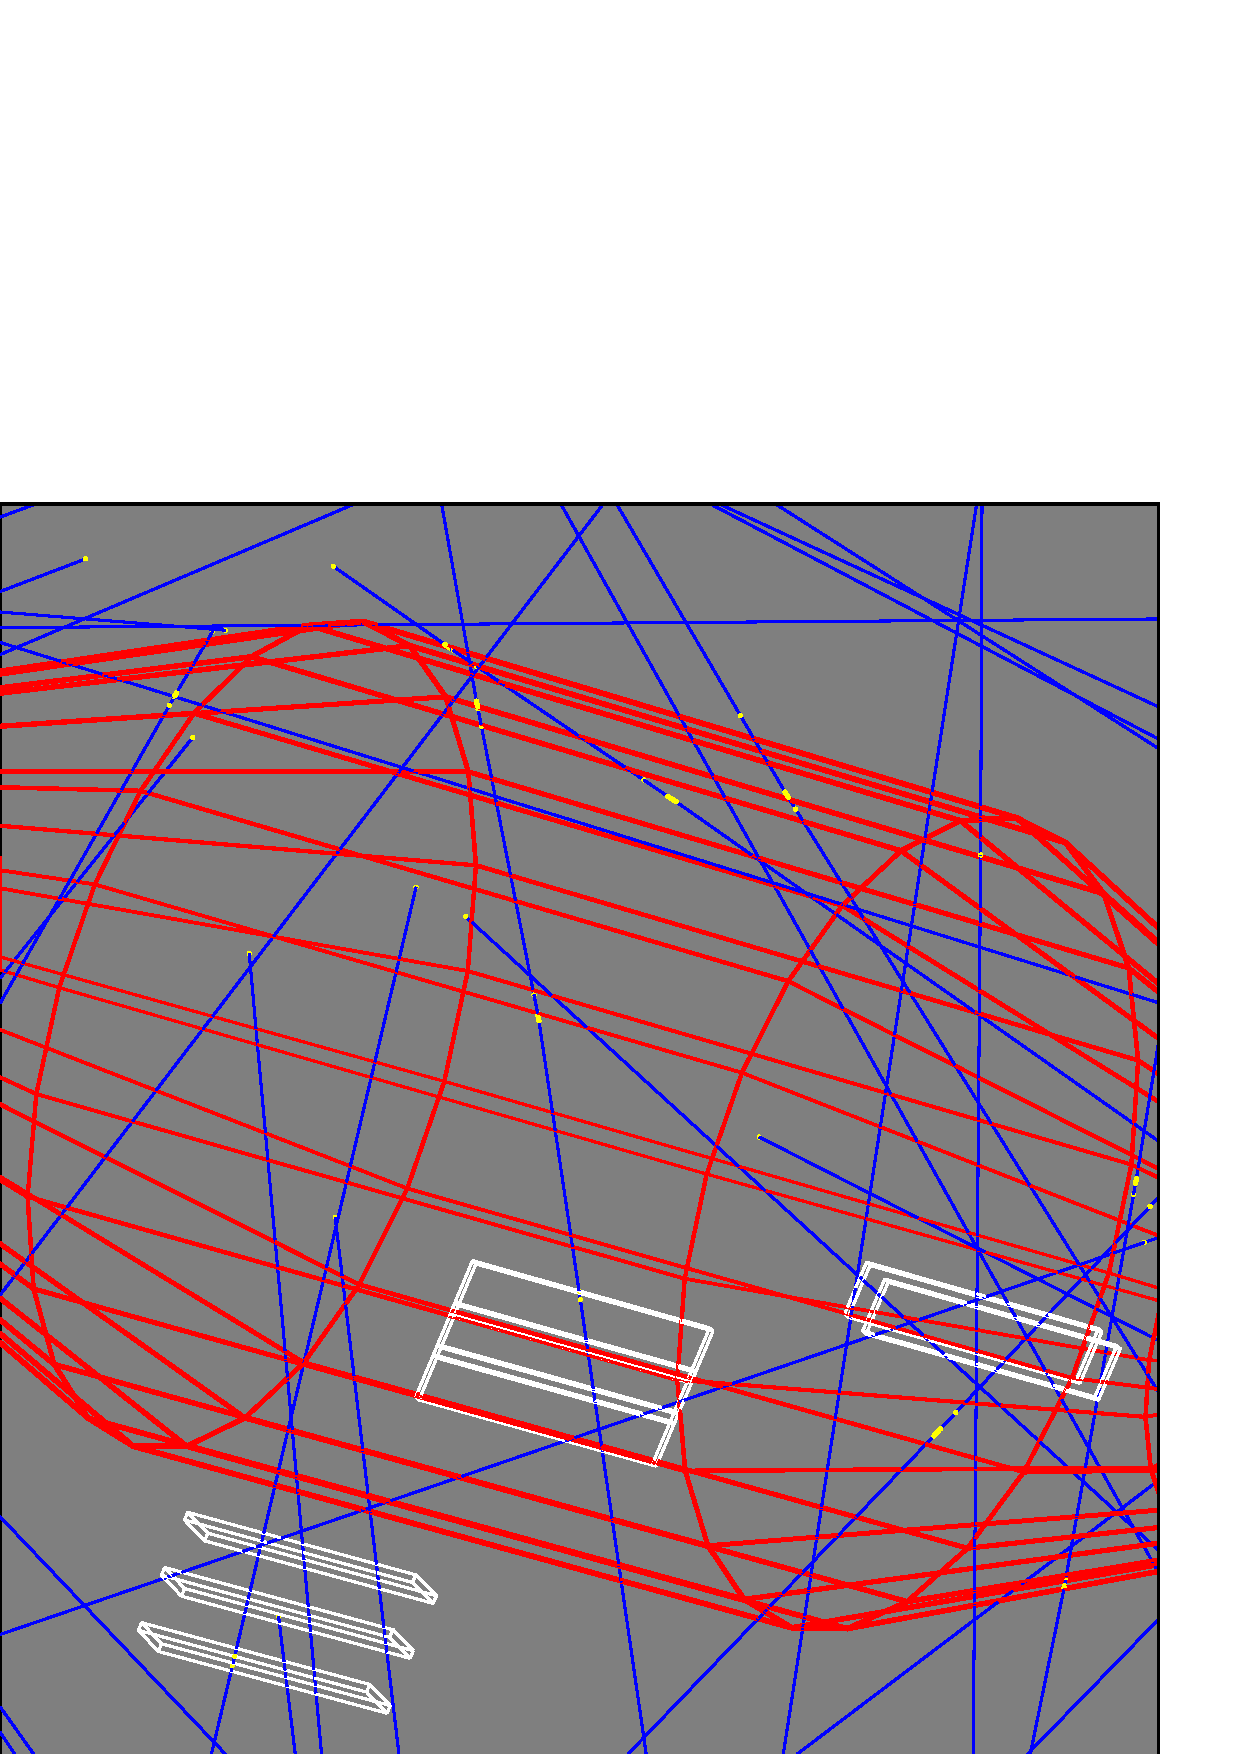
\includegraphics[width = 0.5\textwidth]{graphics/simulation/moduleHit.png}
  	\caption[Simulation geometry setup]{Screenshot of the geometry setup and muon paths in the OpenGL viewer. The view is upwards through the main spectrometer standing on the west side of it. The three groups of muon modules (white) are visible right below the large main spectrometer structure (red). A variety of incident muons is shown (blue). Hits are marked (yellow) by the Geant4 viewer. A single muon's hits are marked with black circles. Both entry and exit point into and out of the main spectrometer and the detection point are visible.}
  	\label{fig:geant:geometry}
  \end{figure}

  
  %% ===========================
  \section{Muon Generator}
  \label{ch:Simulation software:sec:Muon generator}
  %% ===========================  
  
  The muon generation was realized through the primary generator action. The angular distribution suggested by Henrik Arlinghaus \cite{DTArlinghaus} was implemented. The angular rate dependence is shown in \ref{fig:rateDependance}. The energy was set to \todo{reasonable value} disregarding the actual energy distribution as this was mainly about flight paths that are not strongly dependent on energy at high energies. Starting positions were spherically distributed, with the direction towards the origin, which is in the center of the main spectrometer. Starting positions were then randomly moved in a volume surrounding the spectrometer to account for the non-point like structure of the detection system as a whole, while the distribution describes a single point in space.
  \begin{figure}
  \centering
  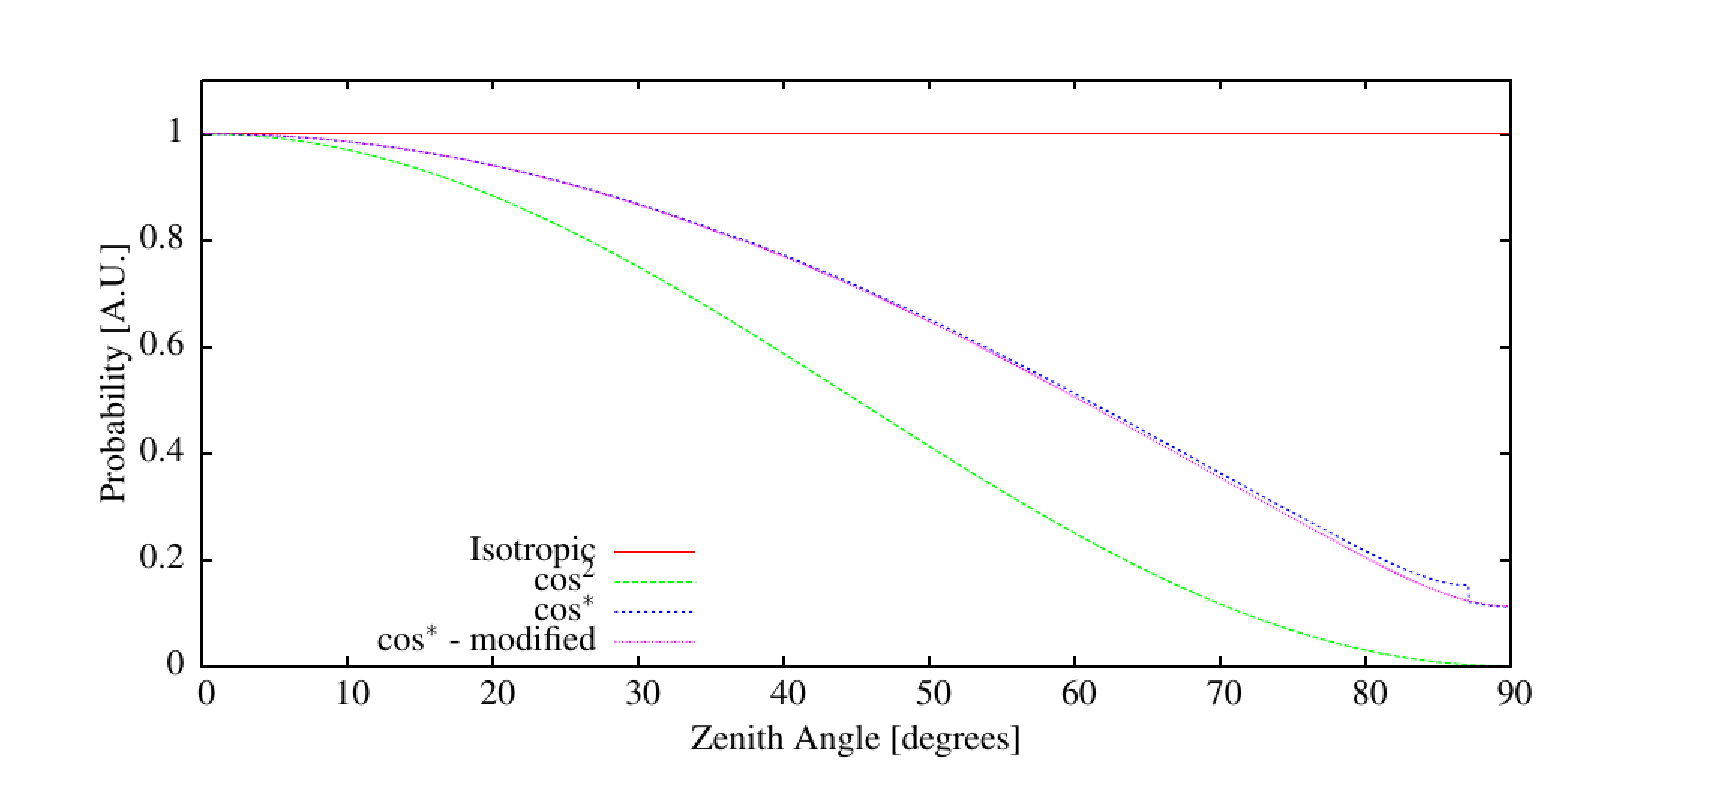
\includegraphics[width = 0.8\textwidth]{graphics/simulation/angularDistributions.eps}
  	\caption[Muon rate dependance on zenith angle]{Different angular distributions. Isotropic and $\cos^2$ distributions are shown opposed to the $\cos^*$ distribution. The latter is plotted with and without a wrongly published parameter from the original publication \cite{distro}.}
  	\label{fig:rateDependance}
  \end{figure}
  The distribution used is the cos* distribution.
  \begin{equation}
  	\cos^*{\left(\theta \right)} = S(\Theta)\cos^{**}{\left(\theta\right)}
  \end{equation}
  with
  \begin{equation}
  	S(\theta) = 0.986 + 0.0007\sec{\theta}
  \end{equation}
  and $S(\theta)$ described by a polynomial
  \begin{equation}
  	\cos^{**} = \sum_{i=0}^{4}{c_i \cos^i{\theta}}.
  	\label{eq:coeffs}
  \end{equation}
  The coefficients are defined differently for different angular ranges shown in table \ref{tab:coefficients}.
  \begin{table}
  \centering
  	\begin{tabular}{|c|c|c|c|c|c|c|}
  	\hline
  		$\cos{\left(\theta\right)}$ & $c_0$ & $c_1$ & $c_2$ & $c_3$ & $c_4$ & max. rel. error\\
  		\hline
  		0 - 0.002 & 0.11137 & 0 & 0 & 0 & 0 & 0.004\\
	
  		0.002 - 0.2 & 0.11148 & -0.03427 & 5.2053 & -14.1971 & 6.138 & 0.3\\
  		0.2 - 0.8 & 0.06714 & 0.71578 & 0.42377 & -0.19634 & -0.021145 & 0.7\\
  		\hline
  	\end{tabular}
	\caption[Angular distribution coefficients]{These are the coefficients for equation \ref{eq:coeffs}. Every set of coefficients is applicable to a certain angular region indicated in the first column. The last column shows the largest occurring relative error in each region. }
  \end{table}

  
  %% ===========================
  \section{Hit Counter}
  \label{ch:Simulation software:sec:Hit counter}
  %% ===========================
  
  To compare moun measurements and simulations, events with at least one module hit were counted.  This made it possible to compare the rates of the single modules, showing that the generator works fine. furthermore, it allowed for a estimation of muons hitting the modules compared to the total of inciding muons. Table \ref{tab:simResults} shows the result of a simulation generating \SI{e 6}{} particles and compares it to measured data. Of the particles generated, the single modules were hit \SI{506\pm 44}{} times. In the same period, the main spectrometer was hit almost \SI{6e4}{} times. This shows formidably that the detection system is by no means a veto system to discriminate muon induced events, but merely for background studies. To compare simulation to real data, a time scale had to be introduced. The nuber of events for a single module corresponds very well to \SI{2}{\second} of measurement time. Consequently, the simulation has been compared to the \SI{2}{\second} average of a half hour run. 
  \begin{table}
  \centering
  	\begin{tabularx}{0.7\textwidth}{|c|>{\centering\arraybackslash}X>{\centering\arraybackslash}X>{\centering\arraybackslash}X>{\centering\arraybackslash}X|}
  	\hline
  	module & 1 & 2 & 3 & 4\\
  	\hline
  	simulation & 550 & 534 & 499 & 410  \\
  	real data & 495$\pm$ 23 & 544 $\pm$ 24 & 497 $\pm$23 & 483$\pm$22 \\
	\end{tabularx}
	\begin{tabularx}{0.7\textwidth}{|c|>{\centering\arraybackslash}X>{\centering\arraybackslash}X>{\centering\arraybackslash}X>{\centering\arraybackslash}X|}
  	\hline
  	module  & 5 & 6 & 7 & 8 \\
  	\hline
  	simulation & 508 & 543 & 506 & 496 \\
  	real data & 490$\pm$23 & 498$\pm$23 & 510$\pm$ 23& 532$\pm$ 24 \\
  	\hline
  	\hline
	\end{tabularx}
  	\begin{tabularx}{0.7\textwidth}{|c|>{\centering\arraybackslash}X>{\centering\arraybackslash}X>{\centering\arraybackslash}X>{\centering\arraybackslash}X>{\centering\arraybackslash}X|}
  	modules & 1+2 & 6+7 & 7+8 & 6+7 & 6+7+8 \\
  	\hline
  	simulation & 204 & 135 & 130 & 66 & 66 \\
  	real data  & 191$\pm$14 & 136$\pm$12 & 146$\pm$12 & 65$\pm$8 & 62$\pm$8 \\
  	\hline
  	\end{tabularx}
  	\caption[Simulation comparison]{Comparison of the simulation data to ral data. }
	\label{tab:simResults}
  \end{table}
  Especially important is that the ratio of multi-module events to single module events is comparable. This can be used as a direct validation of the simulation's angular distribution. The different distances between the single modules are responsible for the difference in counts for multi-module events.
  The ratios are shown in table \ref{tab:}
  \begin{table}
  \centering
  \begin{tabular}{|l|c|c|c|c|c|}
  
  \hline
  	\rule{0pt}{4ex} ratio &$N_{12}/\bar N_{single} $&$ N_{67}/\bar N_{single}$ & $N_{78}/\bar N_{single} $& $N_{68}/\bar N_{single} $& $N_{678}/\bar N_{single}$\\
  	\hline
	simulation & 0.40 & 0.13 & 0.27 & 0.13 & 0.26\\
	real data & 0.38 & 0.27 & 0.29 & 0.13 & 0.12 \\
	\hline
  	\end{tabular}
  	\caption[Single \& Multi side event ratio]{The ration of a multi-module event is compared to the average rate of the single modules. Simulation and real data show comparable values.}
  \end{table}

  The simulation data can be used to estimate the probability of a muon inducing an electron at the detector after taking long term measurements with high statistics.
  Furthermore, by saving entry and exit points to ant out of the main spectrometer, a heatmap of the main spectrometer can be made. Particle tracking from these points with the already avaliable Kassiopeia software will provide more information on and improve the understanding of the background process.
  
  
  
  
  
%% conclusion.tex
%%

%% ==================
\chapter{Conclusion}
\label{ch:Conclusion}

\chapter{Outlook}
\label{ch:Outlook}
%% ==================

\dots



%% --------------------
%% |   Bibliography   |
%% --------------------
\cleardoublepage
\phantomsection
\addcontentsline{toc}{chapter}{\bibname}

\iflanguage{english}
{\bibliographystyle{unsrt}}	% english style
{\bibliographystyle{babalpha-fl}}	% german style
												  
% Use IEEEtran for numeric references
%\bibliographystyle{IEEEtranSA})

\bibliography{thesis}

%% ----------------
%% |   Appendix   |
%% ----------------

\cleardoublepage

%% appendix.tex
%%

%% ==============================
%\chapter{Appendix}
%\label{ch:Appendix}
%% ==============================

\appendix

\iflanguage{english}
{\addchap{Annex}}	% english style
{\addchap{Anhang}}	% german style

\setcounter{figure}{0}


\section{ORCA air coil script}
\label{ch:appendix:sec:orcaScript}
\begin{verbatim}
// import functions for SDS hardware access

#import "~/katrin/ORCARunControl/libs/SDS_RunControl.lib"

#import "~/katrin/ORCARunControl/libs/SDS_AirCoils.lib"



function main(){

//ramp through tenths of the maximum air coil values

for(a=0;a<11; a++){

max=70;

//queue coils 1, 13 and 14 (70A max)

queueAirCoilCurrent_A(1,a*max/10);

queueAirCoilCurrent_A(13,a*max/10);

queueAirCoilCurrent_A(14,a*max/10);

max=100;

//queue coils 2 - 12 (100A max)

for(i=2;i<13;i++){

queueAirCoilCurrent_A(i, a*max/10);

}

//set queued values

sendQueue();

//wait till set

sleep(300);

//output of values

print readAllAirCoilCurrents_A();

sleep(1500);

}

// send the queue of all set points



}
\label{}
\end{verbatim}

\clearpage
\section{Connection scheme DAQ \& high voltage settings}

    \begin{table}[h]
  \centering
  	\begin{tabular}{|c|c|c|c|c|c|}
  	\hline
  		V0 & I0 & I1 & V1 & Ramp Up & Ramp Down\\
  		\hline
  		\SI{1.5}{\kilo\volt} or \SI{1.6}{\kilo\volt} & \SI{2000}{\milli\ampere} & & & \SI{50}{\volt} & \SI{100}{\volt}\\
  		\hline
  	\end{tabular}
  	\caption[High voltage settings]{High voltage settings as used for the muon modules. Modules XX and XX are set to \SI{1.6}{\kilo\volt}.}
  	\label{tab:HVSettings}
  \end{table}
\begin{table}[h]
  	\centering
  	\begin{tabular}{| l | c c | c c | c c | c c |}
  	\hline
  		Module	& 1A	& 1B	& 2A	& 2B	& 3A	& 3B	& 4A	& 4B 	\\
  		Card	& 3	& 3	& 3	& 3	& 6	& 6	& 6	& 6	\\
  		Channel	& 0	& 14	& 3	& 7	& 0	& 14	& 3	& 7	\\
  		HV		& W0 & W1 & W2 & W3 & W4 & W5 & W6 & W7 \\
  		\hline \hline
  		Module	&5A	& 5B	& 6A	& 6B	& 7A	& 7B	& 8A	& 8B	\\
  		Card	& 6	& 6	& 8	& 8	& 8	& 8	& 8	& 8	\\
  		Channel	& 9	& 23	& 0	& 14	& 3	& 7	& 9	& 23	\\
  		HV		& W8 & W9 & E0 & E1 & E2 & E3 & E4 & E5\\
  		\hline
  	\end{tabular}
  	
  	\caption[Main spectrometer DAQ channel assignment]{Assignment of main spectrometer module sides to FLT cards and their channels.}
  	\label{tab:connectionsModulesCards}
  \end{table}
  \begin{figure}[H]
	\centering
  	\includegraphics[width = \textwidth]{graphics/muonModules/mainSpec/FLTback.png}
  	\caption[FLT connector card]{One of the connector cards used at the muon DAQ. The overlayn numbers correspond to the channels accessed via the corresponding connector. Note the non trivial behaviour on le left end. The white labels A, B and C mark the channels used for connecting the muon modules.}
  	\label{fig:FLTback}
  \end{figure}
  

\clearpage
% 
% \begin{figure}
% \centering
% 	\includegraphics[width = 0.9\textwidth]{graphics/monSpec/nonAxiallySym/{+50_12.5_12.5}.eps}
% 	\caption[\SI{50}{\ampere} loops]{Two horizontal loops at \SI{50}{\ampere} current. For all settings see \ref{tab:analysis:nonAxiallySymmetricField}, line 1.}
% 	\label{fig:nonAxiallySym:+50_12.5_12.5.eps}
% \end{figure}
% 
% \begin{figure}
% \centering
% 	\includegraphics[width = 0.9\textwidth]{graphics/monSpec/nonAxiallySym/{+50_12.5_12.5}.eps}
% 	\caption[\SI{50}{\ampere} loops]{Two horizontal loops at \SI{50}{\ampere} current. For all settings see \ref{tab:analysis:nonAxiallySymmetricField}, line 1.}
% 	\label{fig:nonAxiallySym:+50_12.5_12.5.eps}
% \end{figure}
% 
% \begin{figure}
% \centering
% 	\includegraphics[width = 0.9\textwidth]{graphics/monSpec/nonAxiallySym/{+50_12.5_12.5}.eps}
% 	\caption[\SI{50}{\ampere} loops]{Two horizontal loops at \SI{50}{\ampere} current. For all settings see \ref{tab:analysis:nonAxiallySymmetricField}, line 1.}
% 	\label{fig:nonAxiallySym:+50_12.5_12.5.eps}
% \end{figure}


\section{Weather data Christmas 2012}
\label{ch:appendix:sec:weather}

\begin{table}[h]
	\begin{tabular}{| l | cc | cc| cc |}
	\hline
	Date & T$_{low}$ [K] & T$_{high}$ [K] & p$_{low}$ [kPa] & p$_{high}$ [kPa] & p$_l$ / T$_l$ & p$_h$ / T $_h$ \\
	\hline
	21.12.12 & 274.95 & 281.25 & 1010.10 & 1018.20 & 3.67 & 3.62\\
	22.12.12 & 278.55 & 282.15 & 1009.50 & 1020.60 & 3.62 & 3.62\\
	23.12.12 & 282.85 & 287.25 & 1009.50 & 1013.70 & 3.57 & 3.53\\
	24.12.12 & 277.05 & 287.15 & 1007.40 & 1013.50 & 3.64 & 3.53\\
	25.12.12 & 276.05 & 288.35 & 1004.00 & 1010.30 & 3.64 & 3.50\\
	26.12.12 & 281.25 & 282.85 & 1010.40 & 1016.40 & 3.59 & 3.59\\
	27.12.12 & 280.75 & 283.25 & 1004.80 & 1014.70 & 3.58 & 3.58\\
	28.12.12 & 279.65 & 281.85 & 1016.20 & 1029.50 & 3.63 & 3.65\\
	29.12.12 & 276.05 & 284.55 & 1014.90 & 1026.00 & 3.68 & 3.61\\
	30.12.12 & 279.05 & 282.85 & 1015.90 & 1024.60 & 3.64 & 3.62\\
	31.12.12 & 277.05 & 283.15 & 1011.60 & 1024.40 & 3.65 & 3.62\\
	01.01.13 & 274.45 & 281.45 & 1008.10 & 1016.90 & 3.67 & 3.61\\
	02.01.13 & 272.25 & 279.15 & 1017.50 & 1033.00 & 3.74 & 3.70\\
	03.01.13 & 273.65 & 280.45 & 1033.10 & 1038.30 & 3.78 & 3.70\\
	\hline
	
	\end{tabular}
	\caption[Temperature and pressure Rheinstetten]{Temperature and pressure data from the weather station in Rheinstetten. Daily high and low were given, included are the ratio of pressure and temperature for both the high and the low values. This ratio is proportional to the air's density . Bare in mind that this data is only for the low atmospheric layer and the station is also around \SI{20}{\kilo\meter} away  from the KATRIN muon modules.}
	\label{fig:weatherData}
\end{table}

\clearpage


\section{Other monitor spectrometer settings}
\label{ch:appendix:sec:monSpec}

\begin{table}[h]
			\begin{tabular}{C{\textwidth}}
			{\bf non-axially symmetric magnetic field}\\
		\end{tabular}\\
		\begin{tabularx}{\textwidth}{|>{\centering}X>{\centering}X>{\centering}X>{\centering}X>{\centering}X>{\centering}X>{\centering\arraybackslash}X|}
			\hline
			\centering
			solenoid source &solenoid detector &inner aircoil & outer aircoil &outer cent. aircoil &emcs x	&emcs y\\
			\hline
			25	&25	&7	&-7	&5	&0	&-14\\
			\hline
		\end{tabularx}
		\begin{tabularx}{\textwidth}{|l|X|}
		\hline
			mos00159753- & Two horizontal loops at \SI{100}{\ampere}\\
			mos00159754 &\\
			\hline
			mos00159755-& Two horizontal loops at \SI{-100}{\ampere}\\
			mos00159758 &\\
			\hline
			mos00159759-& No current in horizontal loops - background measurement\\
			mos00159771 &\\
			\hline
			mos00159772-& Two horizontal loops at \SI{100}{\ampere}\\
			mos00159773 &\\
			\hline
		\end{tabularx}
		\vspace{0.5cm}
		
		\begin{tabularx}{\textwidth}{|>{\centering}X>{\centering}X>{\centering}X>{\centering}X>{\centering}X>{\centering}X>{\centering\arraybackslash}X|}
			\hline
			\centering
			solenoid source &solenoid detector &inner aircoil & outer aircoil &outer cent. aircoil &emcs x	&emcs y\\
			\hline
			12.5	&12.5	&3.5	&-3.5	&2.5	&0	&0\\
			\hline
		\end{tabularx}
		\begin{tabularx}{\textwidth}{|l|X|}
			\hline
			mos00160661- & Two horizontal loops at \SI{50}{\ampere}\\
			mos00160666 &\\
			\hline
			mos00160667-&No current in horizontal loops - background measurement\\
			mos00160682 &\\
			\hline
			mos00160684-& Two horizontal loops at \SI{-50}{\ampere}\\
			mos00160687 &\\
			\hline
		\end{tabularx}
		\vspace{0.5cm}
		
		\begin{tabularx}{\textwidth}{|>{\centering}X>{\centering}X>{\centering}X>{\centering}X>{\centering}X>{\centering}X>{\centering\arraybackslash}X|}
			\hline
			\centering
			solenoid source &solenoid detector &inner aircoil & outer aircoil &outer cent. aircoil &emcs x	&emcs y\\
			\hline
			6.2 & 6.2 & 1.7 & -1.7 & 1.2 & 0 & 0\\
			\hline
		\end{tabularx}
				\begin{tabularx}{\textwidth}{|l|X|}
			\hline
			mos00160688- & Two horizontal loops at \SI{25}{\ampere}\\
			mos00160691 &\\
			\hline
			mos00160692-&No current in horizontal loops - background measurement\\
			mos00160706 &\\
			\hline
			mos00160707-& Two horizontal loops at \SI{-25}{\ampere}\\
			mos00160711 &\\
			\hline
		\end{tabularx}
\end{table}

% \begin{figure}
% \centering
% 	\includegraphics[width = 0.9\textwidth]{graphics/monSpec/nonAxiallySym/{+50_12.5_12.5}.eps}
% 	\caption[\SI{50}{\ampere} loops]{Two horizontal loops at \SI{50}{\ampere} current. For all settings see \ref{tab:analysis:nonAxiallySymmetricField}, line 1.}
% 	\label{fig:nonAxiallySym:+50_12.5_12.5.eps}
% \end{figure}
% 
% \begin{figure}
% \centering
% 	\includegraphics[width = 0.9\textwidth]{graphics/monSpec/nonAxiallySym/{-50_12.5_12.5}.eps}
% 	\caption[\SI{-50}{\ampere} loops]{Two horizontal loops at \SI{-50}{\ampere} current. For all settings see \ref{tab:analysis:nonAxiallySymmetricField}, line 3.}
% 	\label{fig:nonAxiallySym:-50_12.5_12.5.eps}
% \end{figure}
% 
% \begin{figure}
% \centering
% 	\includegraphics[width = 0.9\textwidth]{graphics/monSpec/nonAxiallySym/{+25_12.5_12.5}.eps}
% 	\caption[\SI{25}{\ampere} loops]{Two horizontal loops at \SI{25}{\ampere} current. For all settings see \ref{tab:analysis:nonAxiallySymmetricField}, line 2.}
% 	\label{fig:nonAxiallySym:+25_12.5_12.5.eps}
% \end{figure}
% \begin{figure}
% \centering
% 	\includegraphics[width = 0.9\textwidth]{graphics/monSpec/nonAxiallySym/{-25_12.5_12.5}.eps}
% 	\caption[\SI{-25}{\ampere} loops]{Two horizontal loops at \SI{-25}{\ampere} current. For all settings see \ref{tab:analysis:nonAxiallySymmetricField}, line 4.}
% 	\label{fig:nonAxiallySym:-25_12.5_12.5.eps}
% \end{figure}
% \begin{figure}
% \centering
% 	\includegraphics[width = 0.9\textwidth]{graphics/monSpec/nonAxiallySym/{BG_12.5_12.5}.eps}
% 	\caption[\SI{50}{\ampere} loops]{Two horizontal loops at \SI{0}{\ampere} current. For all settings see \ref{tab:analysis:nonAxiallySymmetricField}, line 1.}
% 	\label{fig:nonAxiallySym:BG_12.5_12.5.eps}
% \end{figure}
% 
% \begin{figure}
% \centering
% 	\includegraphics[width = 0.9\textwidth]{graphics/monSpec/nonAxiallySym/{BG_25_25}.eps}
% 	\caption[\SI{50}{\ampere} loops]{}
% 	\label{fig:nonAxiallySym:BG_25_25.eps}
% \end{figure}
% 
\clearpage

%%%%%%%%%%%%%%%%%%%%%%%%%%%%%%%%%%%
%MonSpec
%%%%%%%%%%%%%%%%%%%%%%%%%%%%%%%%%%%%
\section{Monitor spectrometer field setup and analysis}
\label{ch:appendix:sec:A3}


\begin{figure}[H]
\centering

		\centerline{\includegraphics[width = 1.3\linewidth]{graphics/analysis/monSpec/fieldSimulation/AB.eps} }
	
	\caption[Asymmetric field \SI{50}{\ampere}]{Flux tube for a \SI{50}{\ampere} detector solenoid, \SI{-8}{\ampere} outer central air coil current.}
	\label{fig:ABf}

\centering
	\includegraphics[width = 0.9\textwidth]{graphics/analysis/monSpec/AB.eps}
	\caption[\SI{50}{\ampere} loops]{Source solenoid off, detector solenoid at \SI{25}{\ampere}. A peak in time is visible at \SI{1.8}{\micro\second}. }
	\label{fig:AB}
\end{figure}

\clearpage

\begin{figure}[H]
\centering
			\centerline{\includegraphics[width = 1.3\linewidth]{graphics/analysis/monSpec/fieldSimulation/AA.eps}}
	
	\caption[\SI{25}{\ampere} asymmetric]{Flux tube for a \SI{25}{\ampere} detector solenoid.}
	\label{fig:AAf}
\end{figure}

\begin{figure}
\centering
	\includegraphics[width = 0.9\textwidth]{graphics/analysis/monSpec/AA.eps}
	\caption[\SI{25}{\ampere} asymmetric]{Source solenoid off, detector solenoid at \SI{25}{\ampere}}.
	\label{fig:AA}
\end{figure}
\clearpage



\begin{figure}
\centering
	\centerline{\includegraphics[width = 1.3\linewidth]{graphics/analysis/monSpec/fieldSimulation/AC.eps} }
	
	\caption[\SI{50}{\ampere} loops]{Flux tube for a \SI{50}{\ampere} detector solenoid, \SI{-7}{\ampere} outer central air coil current.}
	\label{fig:ACf}
\end{figure}

\begin{figure}
\centering
	\includegraphics[width = 0.9\textwidth]{graphics/analysis/monSpec/AC.eps}
	\caption[\SI{50}{\ampere} loops]{Two horizontal loops at \SI{0}{\ampere} current. Both solenoids at \SI{25}{\ampere}.}
	\label{fig:AC}
\end{figure}
\clearpage






\begin{figure}
\centering
	\centerline{\includegraphics[width = 1.3\linewidth]{graphics/analysis/monSpec/fieldSimulation/AD.eps} }
	
	\caption[\SI{50}{\ampere} loops]{Flux tube for a \SI{50}{\ampere} detector solenoid, \SI{-6}{\ampere} outer central air coil current.}
	\label{fig:ADf}
\end{figure}

\begin{figure}
\centering
	\includegraphics[width = 0.9\textwidth]{graphics/analysis/monSpec/AD.eps}
	\caption[\SI{50}{\ampere} loops]{Two horizontal loops at \SI{0}{\ampere} current. Both solenoids at \SI{25}{\ampere}.}
	\label{fig:AD}
\end{figure}
\clearpage









\begin{figure}
\centering
	\centerline{\includegraphics[width = 1.3\linewidth]{graphics/analysis/monSpec/fieldSimulation/NA.eps} }
	
	\caption[\SI{0}{\ampere} loops]{Two horizontal loops at \SI{0}{\ampere} current. Both solenoids at \SI{25}{\ampere} for a comparison of the background at different field widening.}
	\label{fig:NAf}
\end{figure}

\begin{figure}
\centering
	\includegraphics[width = 0.9\textwidth]{graphics/analysis/monSpec/NA.eps}
	\caption[\SI{0}{\ampere} loops analysis]{Two horizontal loops at \SI{0}{\ampere} current. Both solenoids at \SI{25}{\ampere} for a comparison of the background at different field widening. Some events occur in the expected time window.}
	\label{fig:NA}
\end{figure}
\clearpage



\begin{figure}
\centering
	\centerline{\includegraphics[width = 1.3\linewidth]{graphics/analysis/monSpec/fieldSimulation/NI.eps} }
	
	\caption[\SI{0}{\ampere} loops]{Two horizontal loops at \SI{0}{\ampere} current. Both solenoids at \SI{12.5}{\ampere} for a comparison of the background at different field widening. }
	\label{fig:NIf}
\end{figure}

\begin{figure}
\centering
	\includegraphics[width = 0.9\textwidth]{graphics/analysis/monSpec/NI.eps}
	\caption[\SI{0}{\ampere} loops analysis]{Two horizontal loops at \SI{0}{\ampere} current. Both solenoids at \SI{12.5}{\ampere} for a comparison of the background at different field widening.}
	\label{fig:NI}
\end{figure}
\clearpage



\begin{figure}
\centering
	\centerline{\includegraphics[width = 1.3\linewidth]{graphics/analysis/monSpec/fieldSimulation/NB.eps} }
	
	\caption[\SI{50}{\ampere} loops]{Two horizontal loops at \SI{50}{\ampere} current. Both solenoids at \SI{12.5}{\ampere}. Shift of the flux tube downwards visible.}
	\label{fig:NBf}
\end{figure}

\begin{figure}
\centering
	\includegraphics[width = 0.9\textwidth]{graphics/analysis/monSpec/NB.eps}
	\caption[\SI{50}{\ampere} loops analysis]{Two horizontal loops at \SI{50}{\ampere} current. Both solenoids at \SI{12.5}{\ampere} }
	\label{fig:NB}
\end{figure}
\clearpage





\begin{figure}
\centering
	\centerline{\includegraphics[width = 1.3\linewidth]{graphics/analysis/monSpec/fieldSimulation/NE.eps} }
	
	\caption[\SI{-50}{\ampere} loops]{Two horizontal loops at \SI{-50}{\ampere} current. Both solenoids at \SI{12.5}{\ampere}. Shift of the flux tube upwards visible.}
	\label{fig:NEf}
\end{figure}

\begin{figure}
\centering
	\includegraphics[width = 0.9\textwidth]{graphics/analysis/monSpec/NE.eps}
	\caption[\SI{-50}{\ampere} loops analysis]{Two horizontal loops at \SI{-50}{\ampere} current. Both solenoids at \SI{12.5}{\ampere}.}
	\label{fig:NE}
\end{figure}
\clearpage





\begin{figure}
\centering
	\centerline{\includegraphics[width = 1.3\linewidth]{graphics/analysis/monSpec/fieldSimulation/NC.eps} }
	
	\caption[\SI{25}{\ampere} loops]{Two horizontal loops at \SI{25}{\ampere} current. Both solenoids at \SI{12.5}{\ampere}. Shift of the flux tube downwards visible.}
	\label{fig:NCf}
\end{figure}

\begin{figure}
\centering
	\includegraphics[width = 0.9\textwidth]{graphics/analysis/monSpec/NC.eps}
	\caption[\SI{25}{\ampere} loops]{Two horizontal loops at \SI{25}{\ampere} current. Both solenoids at \SI{12.5}{\ampere}.}
	\label{fig:NC}
\end{figure}
\clearpage








\begin{figure}
\centering
	\centerline{\includegraphics[width = 1.3\linewidth]{graphics/analysis/monSpec/fieldSimulation/ND.eps} }
	
	\caption[\SI{50}{\ampere} loops]{Two horizontal loops at \SI{-25}{\ampere} current. Both solenoids at \SI{25}{\ampere}. Shift of the flux tube upwards visible. }
	\label{fig:NDf}
\end{figure}

\begin{figure}
\centering
	\includegraphics[width = 0.9\textwidth]{graphics/analysis/monSpec/ND.eps}
	\caption[\SI{50}{\ampere} loops]{Two horizontal loops at \SI{-25}{\ampere} current. Both solenoids at \SI{25}{\ampere}. Unexpectedly low counts probably due to a off-detector flux tube. }
	\label{fig:ND}
\end{figure}
\clearpage











\section{Main spectrometer analysis}
\label{ch:appendix:sec:mainSpec}


\section{A vis.mac file}
\label{ch:appendix:sec:vis.mac}

\begin{verbatim}
# Macro file for the visualization setting in the initialization phase 
# of the Geant4 simulation when running in interactive mode
#
# Use this open statement to create an OpenGL view:
/vis/open OGL 600x600-0+0
#
# Disable auto refresh and quieten vis messages whilst scene and
# trajectories are established:
/vis/viewer/set/autoRefresh false
/vis/verbose warnings
#
# Draw geometry:
/vis/drawVolume
#
# Specify view angle and zoom:
/vis/viewer/set/viewpointVector 0 0 1
#/vis/viewer/set/viewpointThetaPhi 40 40
/vis/viewer/zoomTo 2
#
# Specify style (surface, wireframe, auxiliary edges, display limit...)
/vis/viewer/set/style wireframe
/vis/viewer/set/auxiliaryEdge true
/vis/ogl/set/displayListLimit 100000000
#
# Draw smooth trajectories at end of event, showing trajectory points
# as markers 1 pixel wide:
/vis/scene/add/trajectories smooth
/vis/modeling/trajectories/create/drawByCharge
/vis/modeling/trajectories/drawByCharge-0/default/setDrawStepPts true
/vis/modeling/trajectories/drawByCharge-0/default/setStepPtsSize 1
#
# Draw hits at end of event:
/vis/scene/add/hits
#
# To draw only muons:
/vis/filtering/trajectories/create/particleFilter
/vis/filtering/trajectories/particleFilter-0/add mu+
# To superimpose all of the events from a given run:
/vis/scene/endOfEventAction accumulate
#
# Re-establish auto refreshing and verbosity:
/vis/viewer/set/autoRefresh true
/vis/viewer/set/background grey
/vis/viewer/set/projection perspective
/vis/verbose warnings
#
#Generate 5 muon events with the distribution provided in the code
/run/beamOn 5

\end{verbatim}


	


\end{document}
